\documentclass[11pt,a4paper]{article}

\usepackage[utf8]{inputenc}
\usepackage[T1]{fontenc}
\usepackage{lmodern}
\usepackage[margin=2.4cm,top=2.6cm,bottom=2.6cm]{geometry}
\usepackage{amsmath,amssymb}
\usepackage{graphicx}
\usepackage{booktabs}
\usepackage{xcolor}
\usepackage{enumitem}
\usepackage{titlesec}
\usepackage{fancyhdr}
\usepackage[most]{tcolorbox}
\usepackage{caption}
\usepackage[hidelinks]{hyperref}
\usepackage{longtable}

% Image paths are relative to this file's location (report/).
\graphicspath{{../images/}}

\definecolor{ink}{HTML}{1B2430}
\definecolor{accent}{HTML}{2B5D8C}
\definecolor{accentlight}{HTML}{EAF1F8}
\definecolor{warm}{HTML}{B5651D}
\definecolor{warmlight}{HTML}{FBF1E6}
\definecolor{greyline}{HTML}{C9D1D9}
\definecolor{softgrey}{HTML}{F4F6F8}

\color{ink}

\titleformat{\section}{\Large\bfseries\color{accent}}{\thesection}{0.6em}{}
\titleformat{\subsection}{\large\bfseries\color{ink}}{\thesubsection}{0.6em}{}
\titlespacing*{\section}{0pt}{1.6em}{0.7em}

\pagestyle{fancy}
\fancyhf{}
\renewcommand{\headrulewidth}{0.4pt}
\fancyhead[L]{\small\color{accent}Precog Task Report --- MetaFam}
\fancyhead[R]{\small\color{accent}\thepage}

\captionsetup{font=small,labelfont={bf,color=accent}}

% Callout boxes
\newtcolorbox{plain}[1][]{
  colback=accentlight, colframe=accent, boxrule=0pt, leftrule=3pt,
  arc=1pt, left=8pt, right=8pt, top=6pt, bottom=6pt, #1}

\newtcolorbox{why}[1][]{
  colback=warmlight, colframe=warm, boxrule=0pt, leftrule=3pt,
  arc=1pt, left=8pt, right=8pt, top=6pt, bottom=6pt, #1}

\newtcolorbox{jargon}[1][]{
  colback=softgrey, colframe=greyline, boxrule=0.5pt,
  arc=1pt, left=8pt, right=8pt, top=6pt, bottom=6pt, #1}

\newcommand{\rel}[1]{\texttt{\small #1}}

% Each Task restarts its own section/subsection numbering. hyperref anchors
% (\theHsection) stay globally unique via a task counter even though the
% *displayed* numbers (\thesection) reset every task.
\newcounter{tasknum}
\makeatletter
\renewcommand{\theHsection}{tsk\thetasknum.\arabic{section}}
\renewcommand{\theHsubsection}{tsk\thetasknum.\arabic{section}.\arabic{subsection}}
\makeatother
\newcommand{\starttask}[1]{%
  \clearpage
  \stepcounter{tasknum}%
  \setcounter{section}{0}%
  \setcounter{subsection}{0}%
  \section*{#1}%
  \addcontentsline{toc}{section}{#1}%
}

\begin{document}

% ---------------------------------------------------------------- TITLE
\begin{titlepage}
\centering
\vspace*{2.5cm}
{\color{accent}\rule{\textwidth}{2pt}}\\[0.8em]
{\Huge\bfseries Precog Task Report}\\[0.5em]
{\LARGE Aakarsh Mishra \,\textbullet\, 2024111007}\\[0.8em]
{\color{accent}\rule{\textwidth}{2pt}}\\[2.5cm]

{\Large\bfseries\color{accent} META F-A-M-I-L-Y}\\[2cm]

\begin{minipage}{0.82\textwidth}
\begin{jargon}
I covered all tasks mentioned (1, 2, 3 and 4). No bonus parts were
explicitly mentioned in my task. This report aims to cover everything I
have done, and explains all concepts used from the ground up. This report
consists of outputs, visualizations and relevant results from my python
notebooks, along with some theoretical explanations; but does not get into
any of the code whatsoever. Everything marked in blue text is a unique
approach where I felt like I stood out, which I think led to some
interesting results.
\end{jargon}
\end{minipage}

\vfill
{\small Companion to the \texttt{knowledge-graph-exploration} repository}
\end{titlepage}

\tableofcontents

% ================================================================== TASK 1
\starttask{Task 1 --- Dataset Exploration: MetaFam Knowledge Graph}

\section{The MetaFam Dataset}

It is a synthetic (artificially made) family knowledge graph, depicting
family relations in the format of triples --- for example
\rel{(Ram12, sonOf, Shyam13)}. Each person is a vertex; each relation is a
directed edge.

Until Task 4, only \texttt{train.txt} is used, which contains:

\begin{itemize}[leftmargin=1.4em,itemsep=2pt]
\item 13{,}821 triples
\item 1{,}316 unique people
\item 28 unique relation types
\item Average degree (in + out) $\approx 21.0$
\end{itemize}

\section{Relationship Types \& Generation Weights}

\subsection{Relation categories and their distribution}

The 28 relations fall into six broad categories --- Sibling, Parent/Child,
Grandparent, Great-Grand, Aunt/Uncle, and Cousin --- shown in
Figure~\ref{fig:t1-reldist}. The most common relation is \rel{grandsonOf}
(814 occurrences); the rarest is \rel{girlSecondCousinOf} (62).

\begin{figure}[h]
\centering
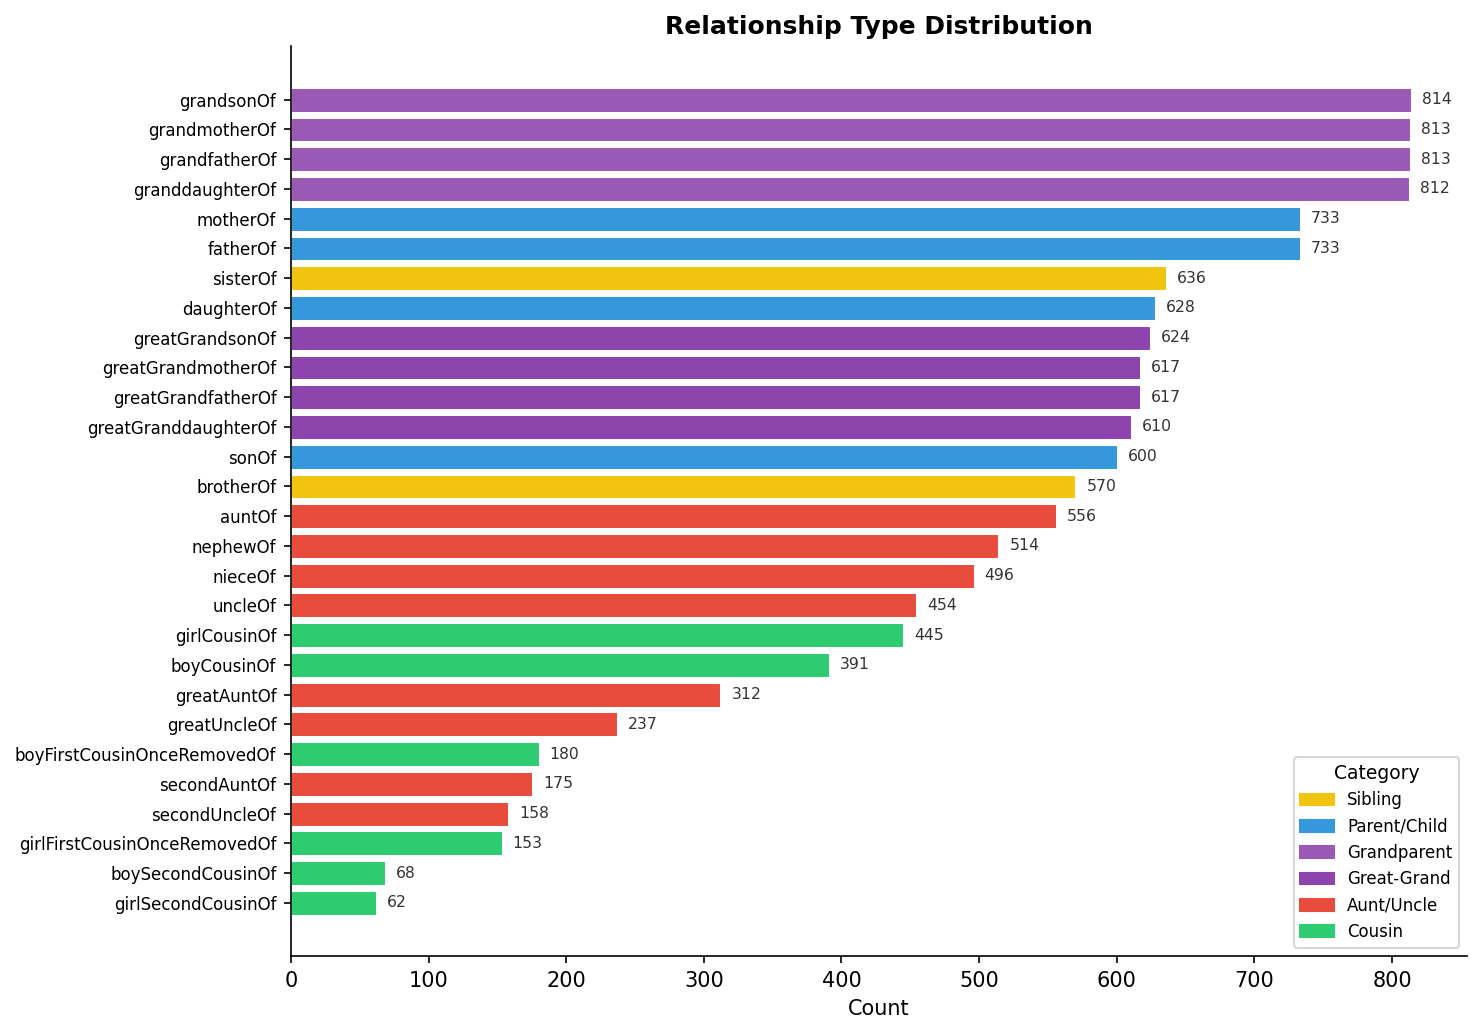
\includegraphics[width=0.82\textwidth]{task1/relation_distribution.png}
\caption{How often each of the 28 relation types appears, coloured by
category. The distribution is heavily skewed toward parent/child and
grandparent relations.}
\label{fig:t1-reldist}
\end{figure}

\subsection{What are generation weights?}

Each relation carries a \emph{generational offset}: \rel{motherOf} is
$+1$ (the head is one generation above the tail), \rel{sonOf} is $-1$,
\rel{sisterOf} is $0$, and so on up to $\pm 3$ for great-grandparent
relations. These weights drive the generation analysis in \S5 and the
community-detection graph construction in Task 2.

\begin{why}
\textbf{A constant that used to disagree with itself.} The generation
weight for \rel{boyFirstCousinOnceRemovedOf} /
\rel{girlFirstCousinOnceRemovedOf} is $-1$, not $0$: Task 3 (\S4.1)
establishes empirically, at 100\% confidence over 64 supporting examples,
that this relation means ``my parent's cousin'' --- a genuine
one-generation gap, not a same-generation relation. An earlier version of
this codebase had the correct $-1$ here but a stray $0$ in a second,
duplicated copy of these weights used for Task 2's graph construction,
which silently zeroed out the generational distance for that relation in
one task but not the other. The weights are now defined in exactly one
place (\texttt{src/metafam.py}) and used by every notebook, so that
particular category of bug --- two copies of the same constant quietly
drifting apart --- cannot recur.
\end{why}

\subsection{Gender Consistency Check}

For my own sake, and as a consistency check, I inferred each person's
gender from every relation where they appear as the head of a gendered
triple (e.g.\ \rel{motherOf} implies female, \rel{sonOf} implies male),
then checked whether any person received conflicting signals.

Sure enough, the graph is gender-consistent: 646 males, 670 females, and
\textbf{zero} conflicts.

\section{Graph Structure Metrics}

\subsection{Degree Distribution}

In a triple \rel{(head, relation, tail)}, the head gets $+1$ out-degree
and the tail gets $+1$ in-degree. In-degree and out-degree distributions
are quite similar, because most relations exist as reciprocal pairs
(\rel{sonOf} / \rel{motherOf}). Total degree (in + out) can exceed family
size because of these reciprocal edges; unique-neighbour count reflects
the actual number of distinct relatives.

\begin{figure}[h]
\centering
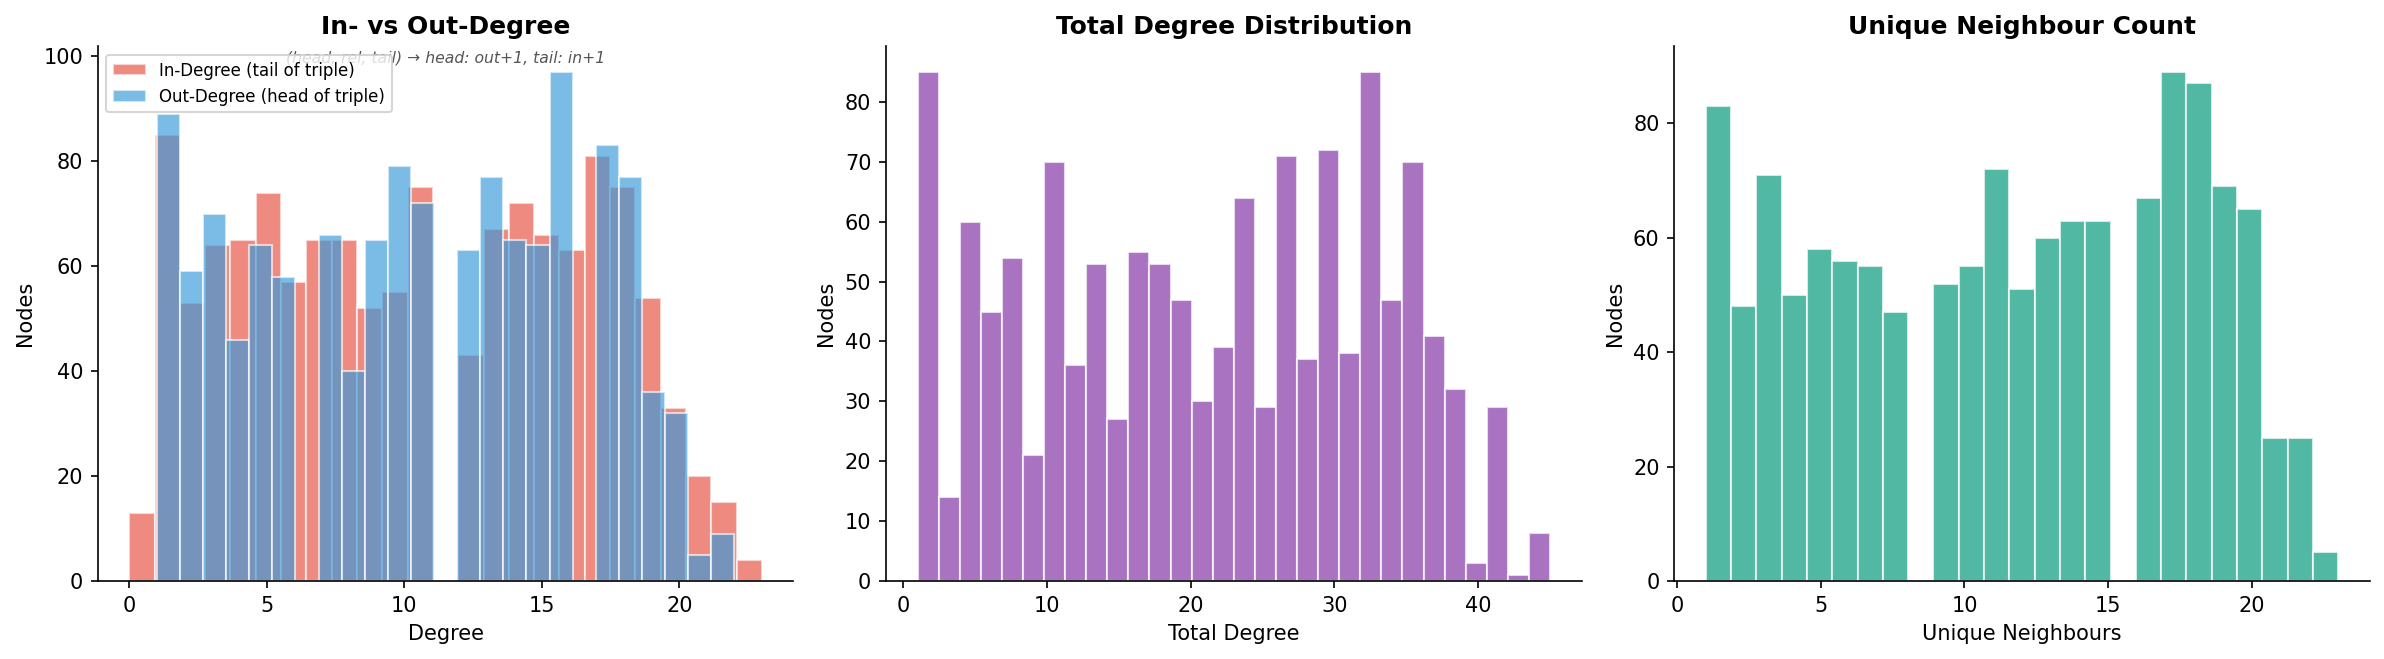
\includegraphics[width=0.92\textwidth]{task1/degree_distribution.png}
\caption{In- vs.\ out-degree, total degree, and unique-neighbour count
across all 1{,}316 people.}
\end{figure}

\subsection{Graph Density}

Density is the fraction of possible edges that actually exist:
$0.008$ (0.8\%), which is very sparse. This happens because the
hierarchical family structure does not connect everyone to everyone ---
and, more fundamentally, because the graph is 50 disjoint pieces (\S3.3):
no person in Family A can ever be adjacent to a person in Family B, so
almost all of the $\binom{1316}{2}$ possible pairs are automatically
non-edges before any family's internal structure is even considered.

\subsection{Connected Components (Families)}

A connected component is a sub-graph where every node can reach every
other. ``Weakly connected component'' is the directed-graph version,
where directed edges are treated as undirected for reachability purposes.

This is a striking result: there are exactly 50 weakly connected
components, each of size 26 or 27 (mean size 26.3, 16 families of size 27
and 34 of size 26). No cross-family edges exist at all --- each family is
a fully independent unit. This single fact --- 50 disconnected pieces ---
is the structural property that recurs across every later task: it makes
community detection trivial (Task 2), it makes Node2Vec's walk parameters
irrelevant (Task 2), and it makes naive random negative sampling too easy
in link prediction (Task 4).

\subsection{Diameter}

The diameter of a graph (here, within one weakly connected component) is
the longest shortest path between any two nodes.

\begin{center}
\begin{tabular}{lc}
\toprule
\textbf{Diameter} & \textbf{Families} \\
\midrule
3 & 25 \\
4 & 23 \\
5 & 2 \\
\bottomrule
\end{tabular}
\end{center}

Even the most distant relatives in a family are only 3--5 hops apart.

\subsection{Clustering Coefficient}

The clustering coefficient of a node measures how much its neighbours are
also neighbours of each other --- ``do your relatives also know each
other?'' The global figure is the average of all local coefficients.

\textbf{Result: 0.7346 --- a high value.} This is the correct reading, and
it is worth being precise about why, because it is easy to state
backwards: MetaFam is not a bare family tree, it is an
\emph{extended-kinship} graph in which siblings, cousins, aunts and
uncles are all explicitly linked to \emph{each other}, not just to a
common ancestor, so triangles are common. This is a separate fact from
the low density in \S3.2: density is low \emph{between} families (they
never touch); clustering is high \emph{within} them (relatives know each
other). Both are true at once, and neither implies ``tree-like.''

\begin{figure}[h]
\centering
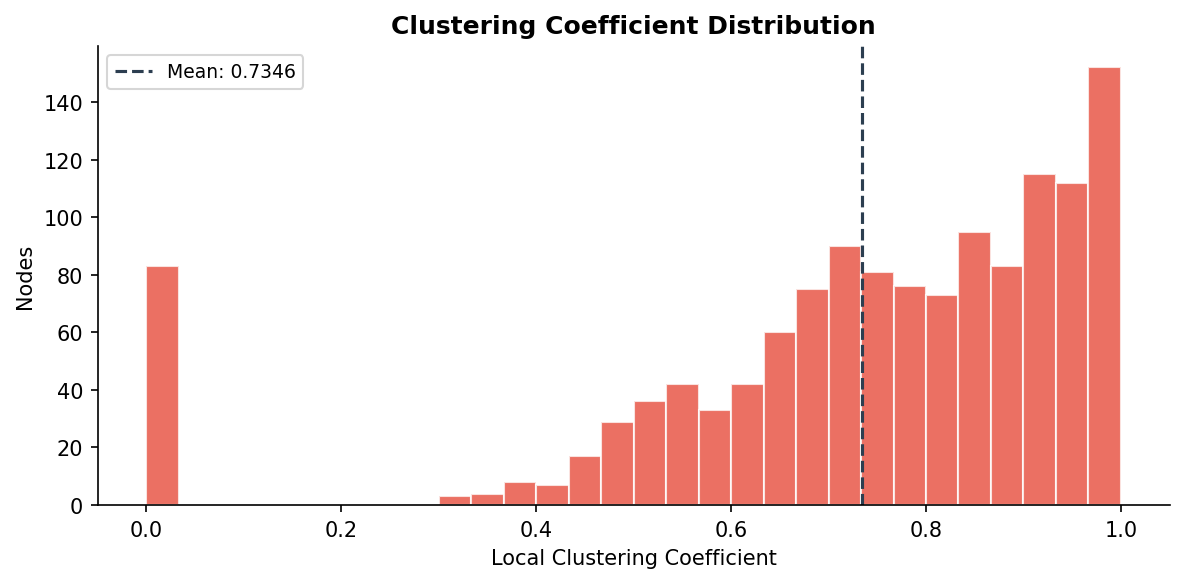
\includegraphics[width=0.7\textwidth]{task1/clustering_distribution.png}
\caption{Distribution of local clustering coefficients. The mean (0.7346)
sits well toward the high end.}
\end{figure}

\subsection{Summary Dashboard}

\begin{figure}[h]
\centering
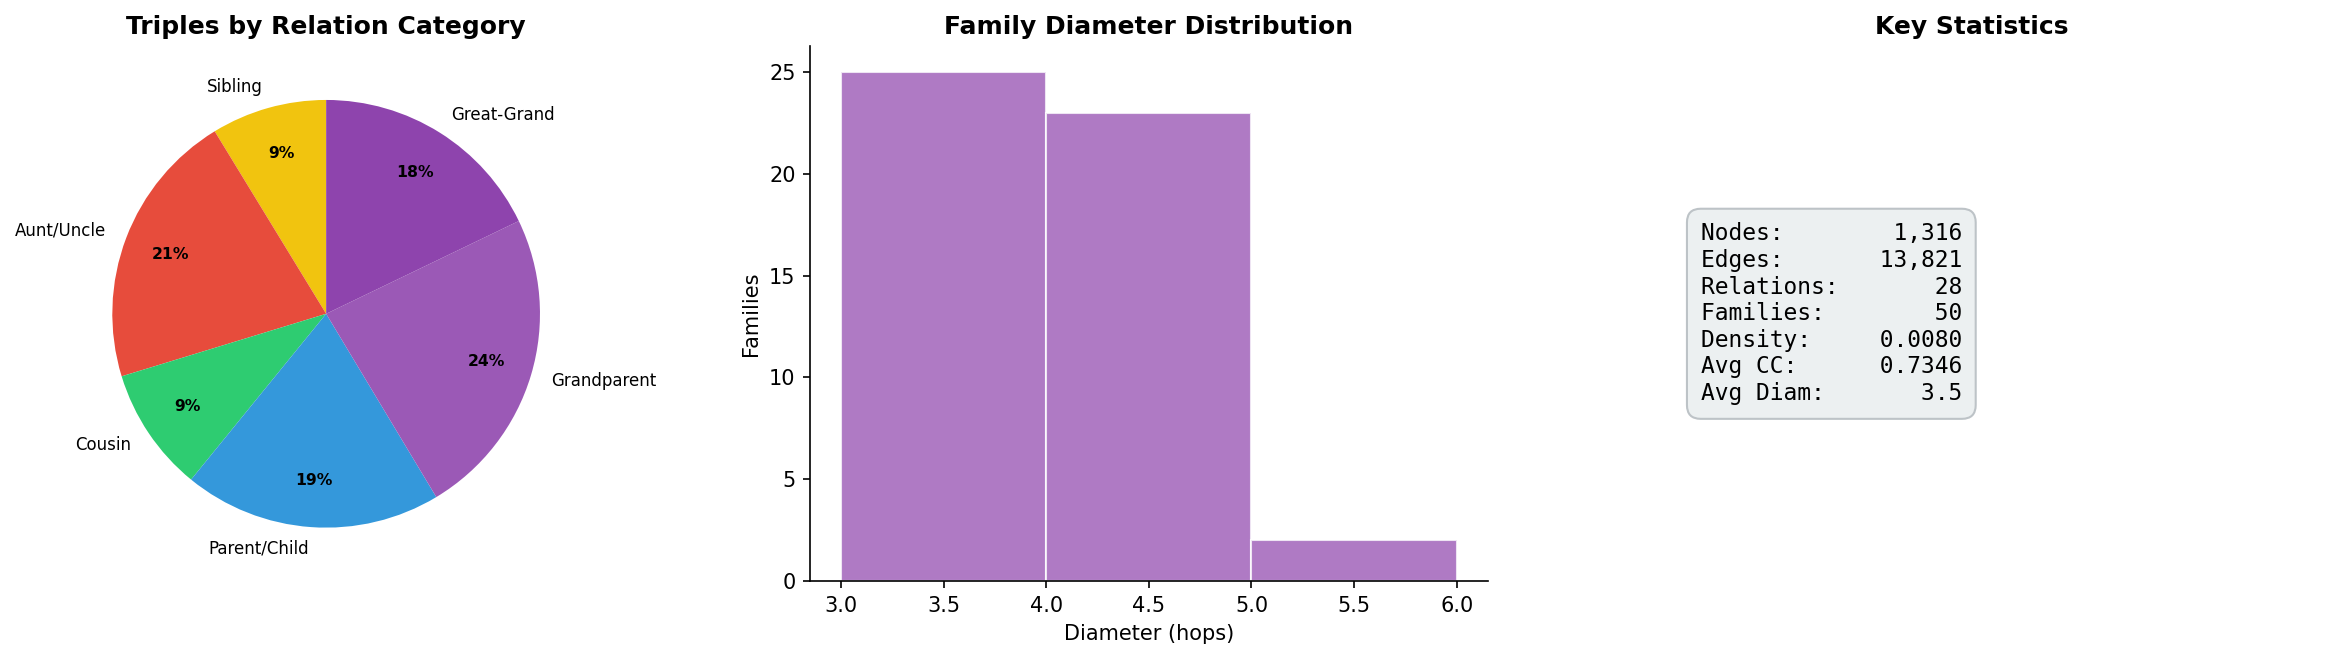
\includegraphics[width=0.95\textwidth]{task1/metrics_dashboard.png}
\caption{Relation-category breakdown, diameter distribution, and headline
statistics in one view.}
\end{figure}

\section{Centrality Analysis --- Who Is ``Important''?}

\subsection{Why centrality matters}

In a family KG, ``importance'' means different things depending on
context, so I use four metrics that each capture a different notion of
it.

\subsection{Closeness Centrality}

The reciprocal of the average shortest-path distance from a person to all
other reachable people. A high score means this person is few hops from
everyone else. People in the ``structural centre'' of the family --- seen
here to be mid-generation parents or grandparents --- score highest,
because they have short paths to both ancestors and descendants.

\subsection{Betweenness Centrality}

The fraction of all shortest paths between any two people that pass
through this specific person. These are the ``bridge'' individuals who
connect different branches of the family tree.

\subsection{PageRank}

Imagine a person randomly following relationship edges through the family
tree; their PageRank score is the probability of being at that person's
node at any given time (a Markov-chain stationary distribution). Parents
and grandparents score highest because they receive many incoming edges
(\rel{motherOf}, \rel{grandfatherOf}, \ldots) from their many descendants.

\subsection{The Broker Score (custom metric)}

\[
\text{Broker}(v) = \deg(v) \times \bigl(1 - \text{clust}(v)\bigr)
\]

A high score requires \emph{high degree} (knows many people) \textbf{and}
\emph{low clustering} (those people don't know each other). This
identifies people who connect otherwise-separate groups --- the same
intuition as betweenness, at a fraction of the computational cost (no
shortest-path search required, just local degree and clustering).

\begin{plain}
\textbf{Extending the Broker Score globally.} The heatmap below analyses
only the largest single family. But because Broker Score is defined
locally (degree and clustering are per-node quantities that make sense
even across disconnected components), it can be computed for
\emph{every} person across all 50 families at once and ranked globally
--- something betweenness centrality cannot do as cheaply, since
betweenness on a disconnected graph has to be computed per component
anyway. The top-20 global brokers span several different families, which
is itself informative: no single family monopolises structural
importance.
\end{plain}

\subsection{Results --- Centrality Heatmap}

\begin{figure}[h]
\centering
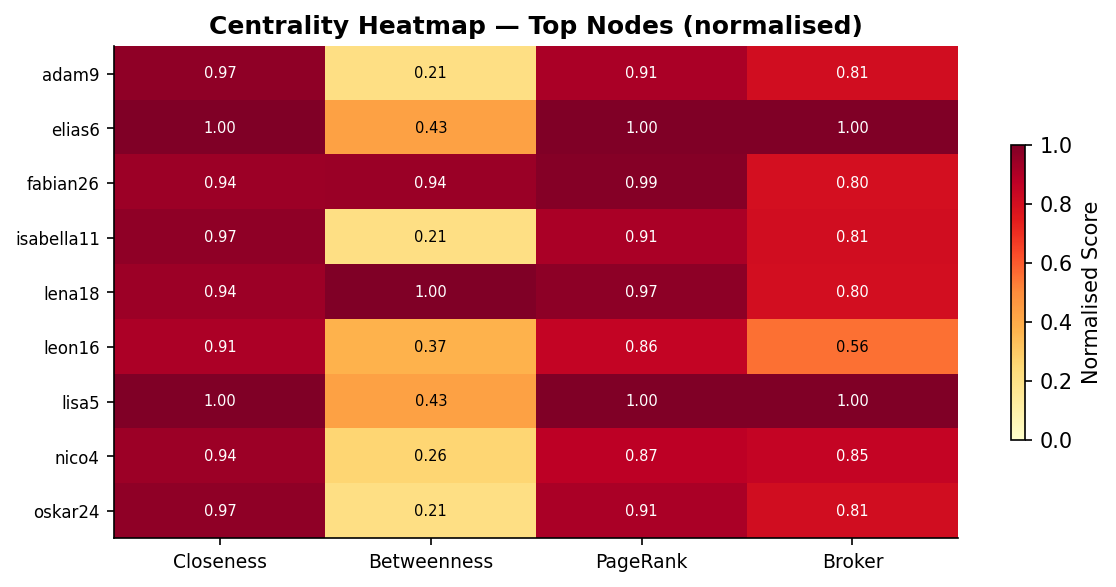
\includegraphics[width=0.85\textwidth]{task1/centrality_heatmap.png}
\caption{Normalised score of the top nodes (by any metric) across all
four centrality measures, largest family.}
\end{figure}

\begin{figure}[h]
\centering
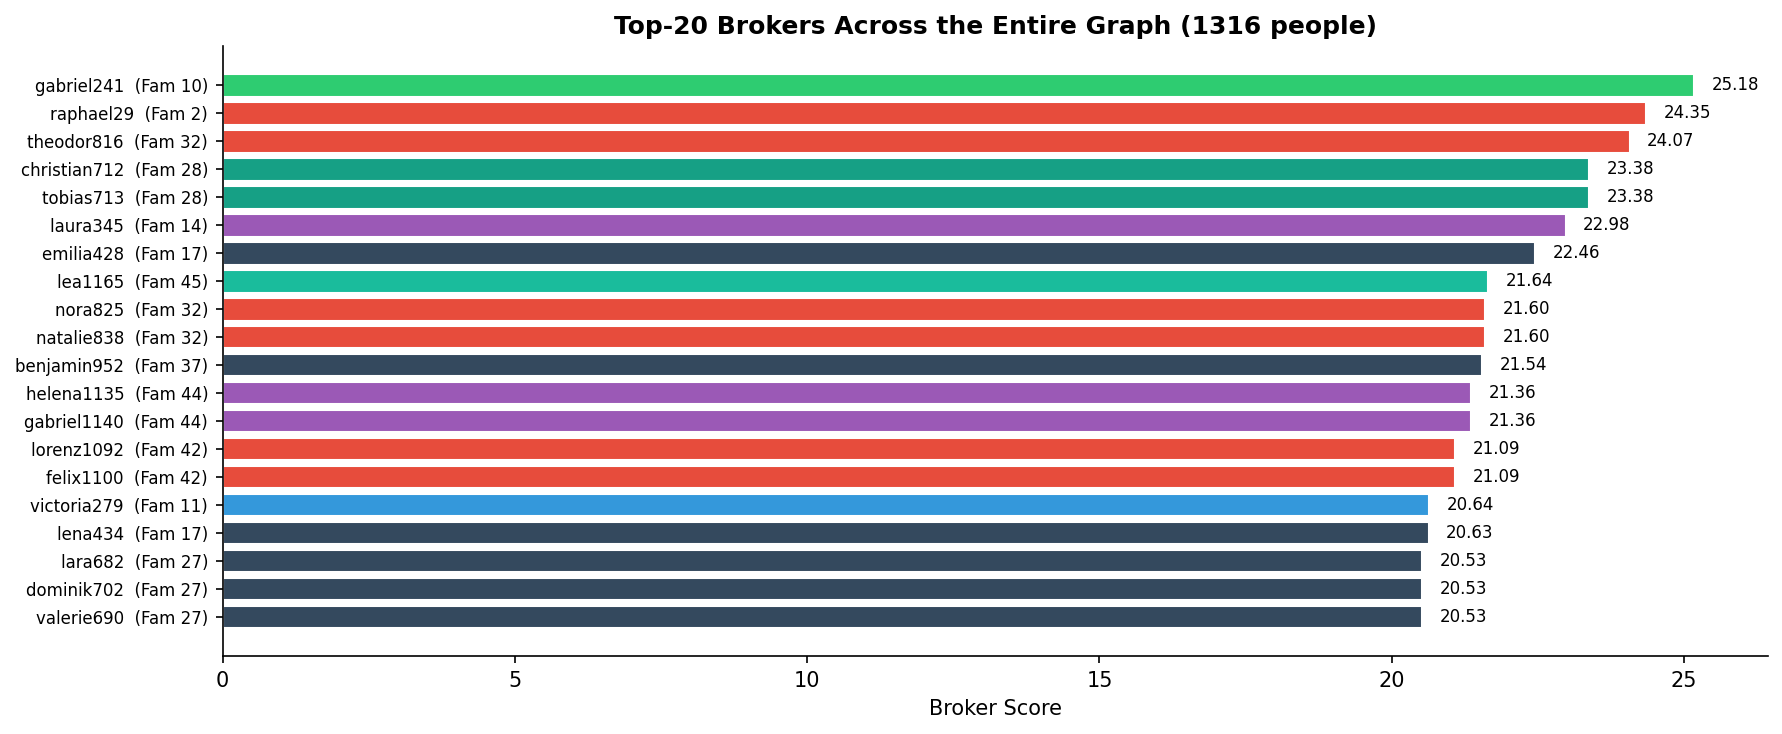
\includegraphics[width=0.92\textwidth]{task1/global_broker_top20.png}
\caption{Top-20 broker scores across the entire graph (all 50 families),
coloured by family.}
\end{figure}

\section{Generation Analysis}

\subsection{Method --- BFS-based generation assignment}

Starting from an arbitrary root node in a family, generation levels
propagate outward via breadth-first search, using the generation weights
from \S2.2: an edge $(u, \text{rel}, v)$ sets
$\text{gen}(v) = \text{gen}(u) - \text{weight}(\text{rel})$ for a
successor and the mirror rule for a predecessor.

\begin{why}
\textbf{This is now checked, not just assumed.} For every directed edge
inside every family, I verify that the assigned generations are
internally consistent with the edge's own relation weight, and count any
violations. Across all 50 families and 13{,}821 directed edges, there are
\textbf{zero} violations --- so ``BFS assigns clean integer levels'' is
now an evidence-backed claim, not an unverified assertion.
\end{why}

\subsection{Generational depth per family}

\begin{figure}[h]
\centering
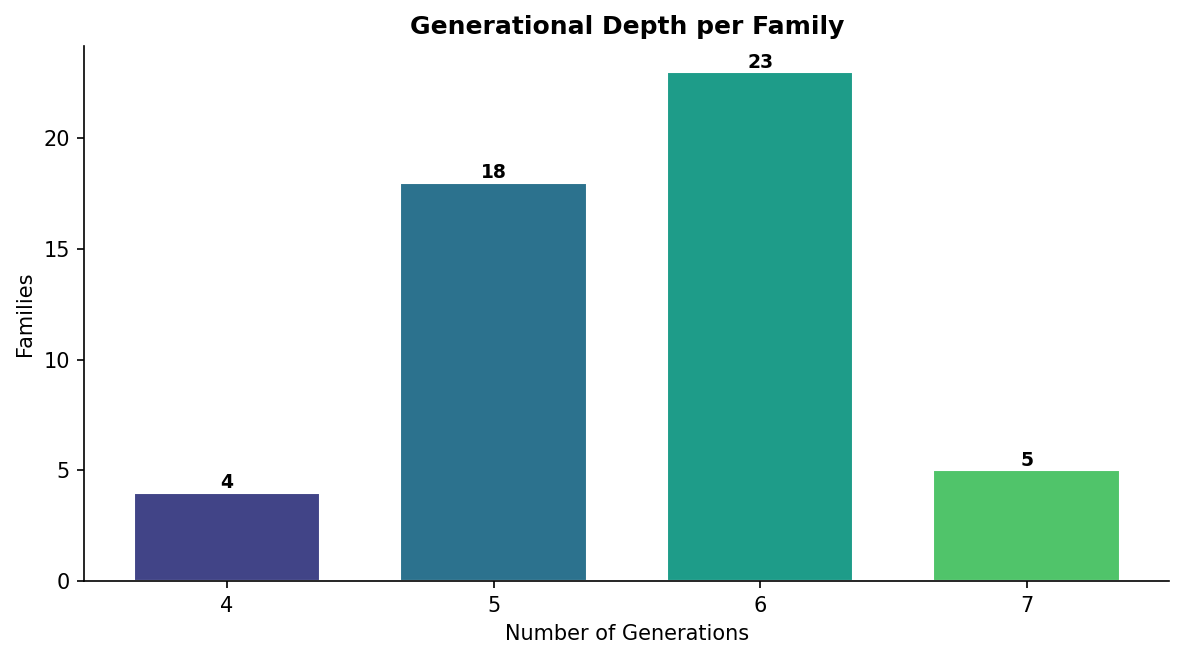
\includegraphics[width=0.62\textwidth]{task1/generation_depth.png}
\caption{Number of distinct generation levels per family; most families
span 5--6 generations (overall range 4--7, mean $\approx 5.6$).}
\end{figure}

\section{Visualizations}

\begin{figure}[h]
\centering
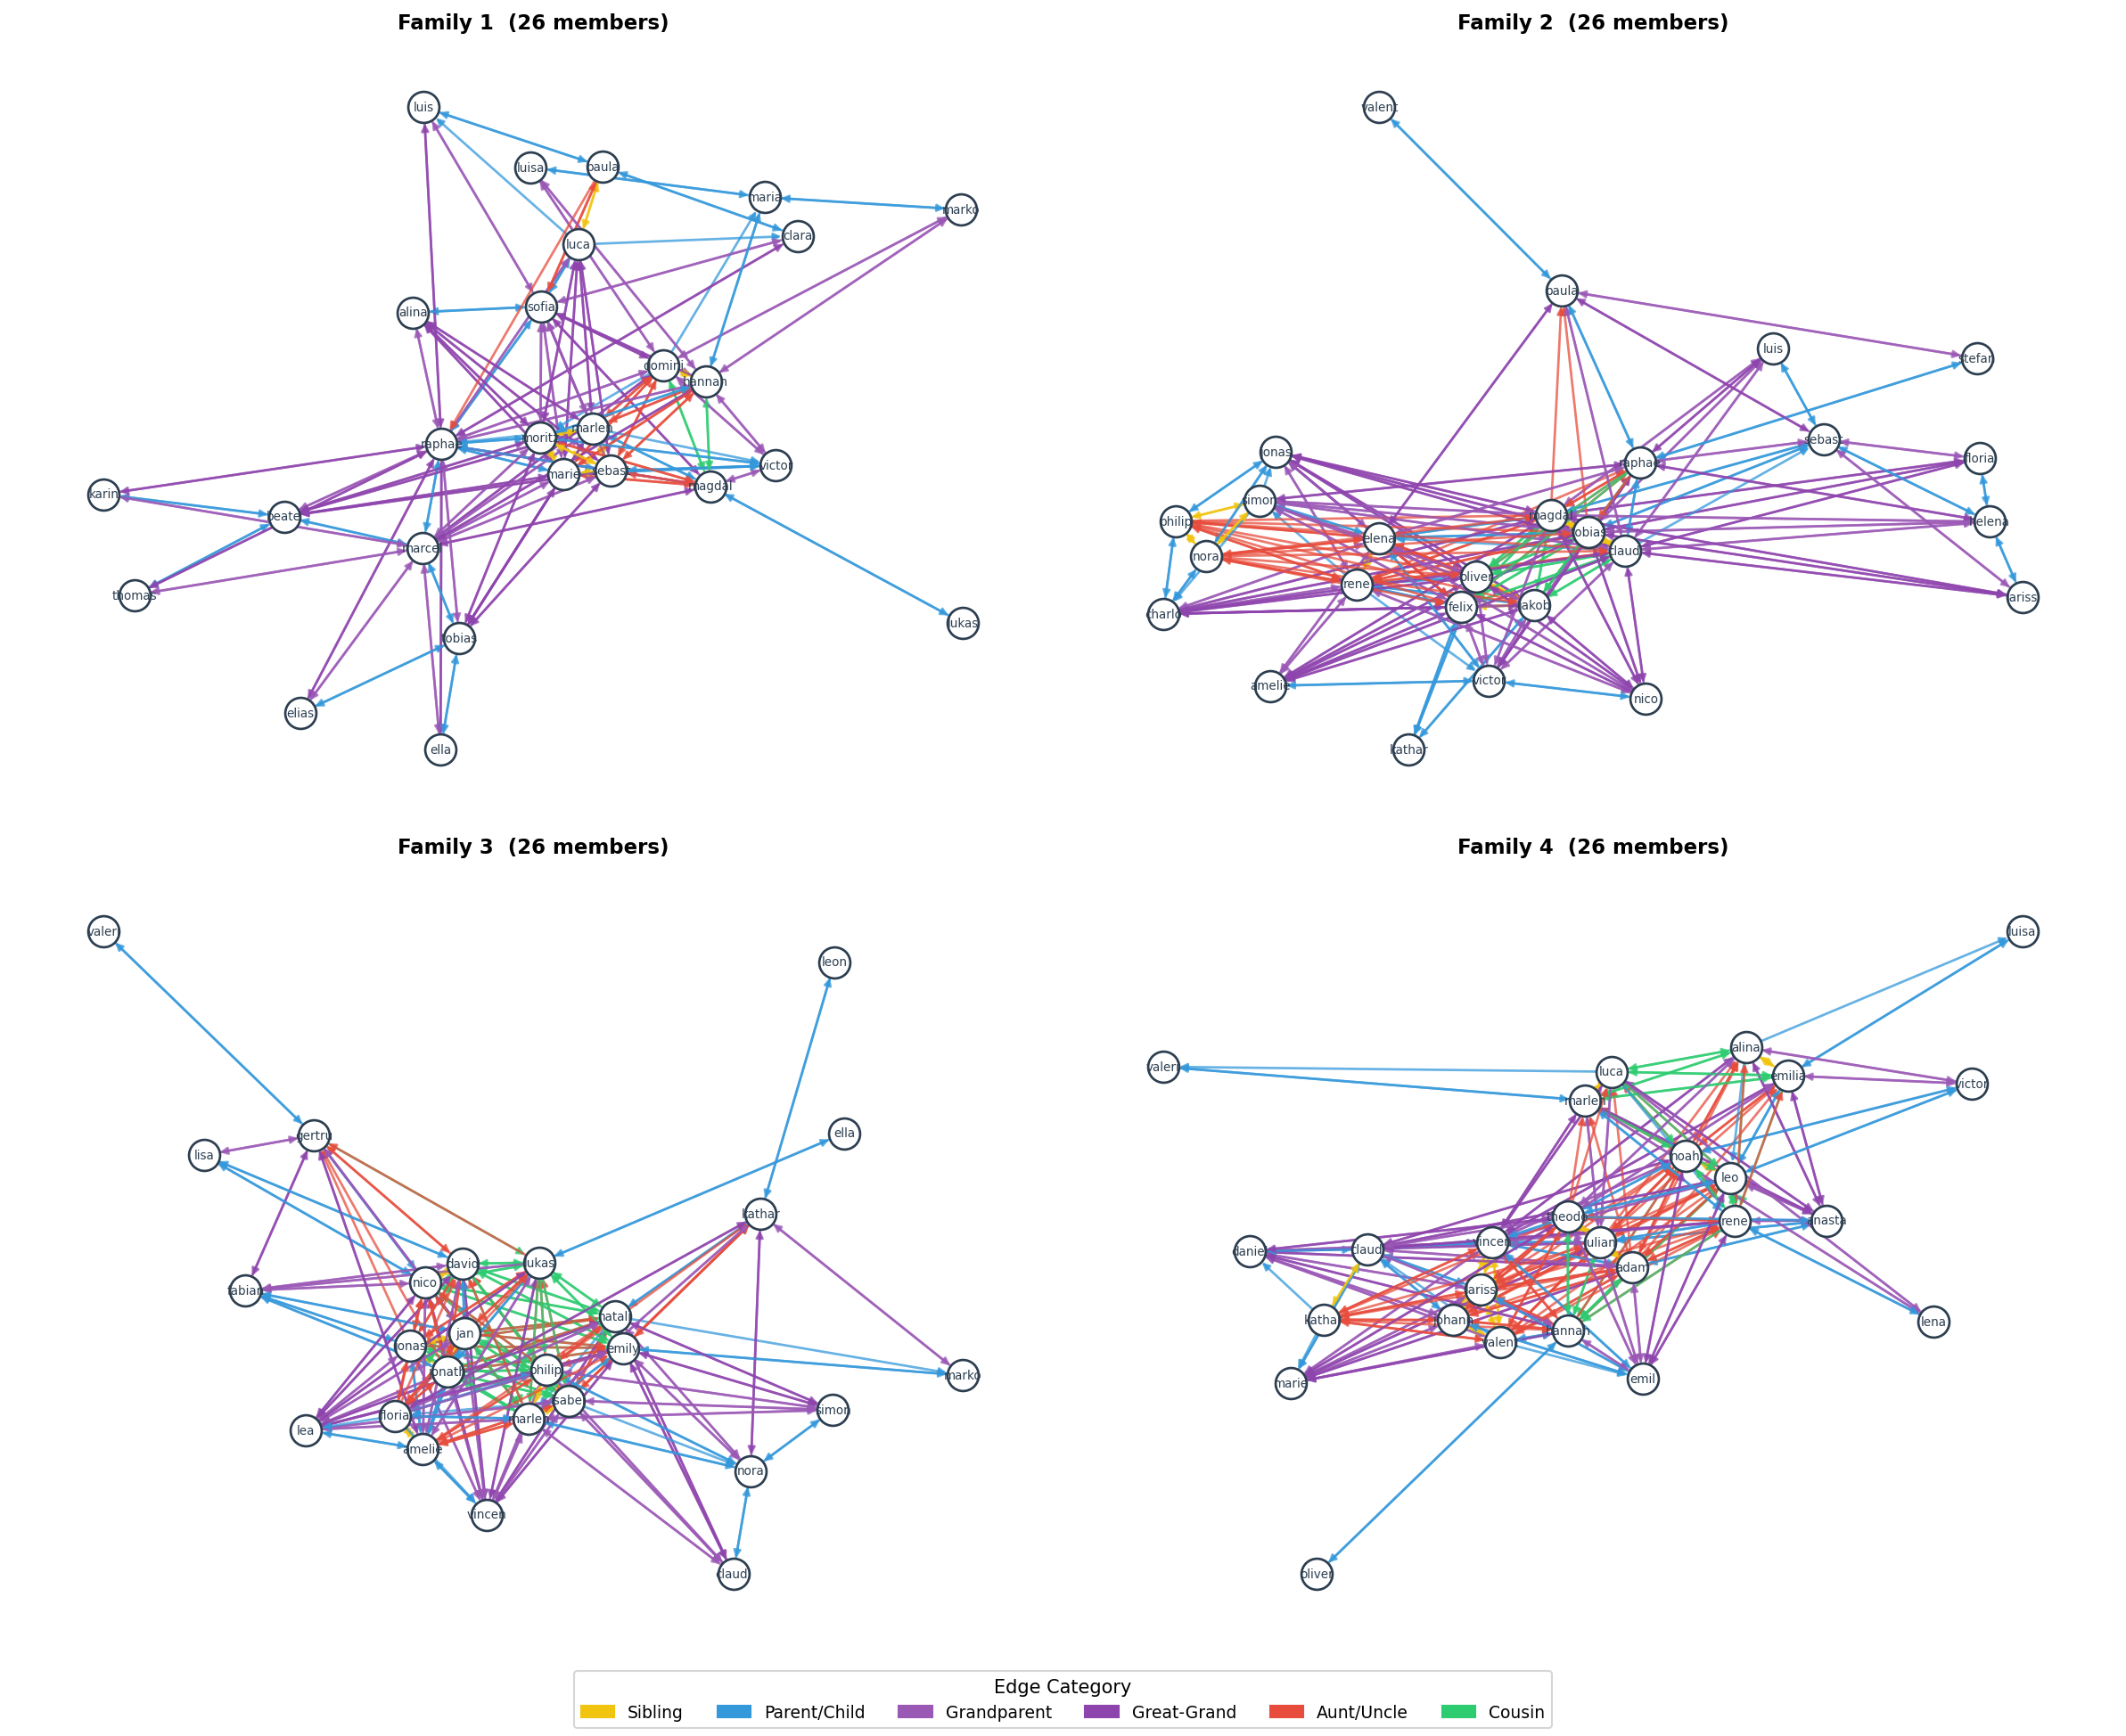
\includegraphics[width=0.95\textwidth]{task1/family_clusters.png}
\caption{Four average-sized family clusters, laid out with a spring
layout weighted so siblings sit close together and distant relatives sit
further apart. Dense cores (siblings and parents) surrounded by
peripheral members are visible in each.}
\end{figure}

\begin{figure}[h]
\centering
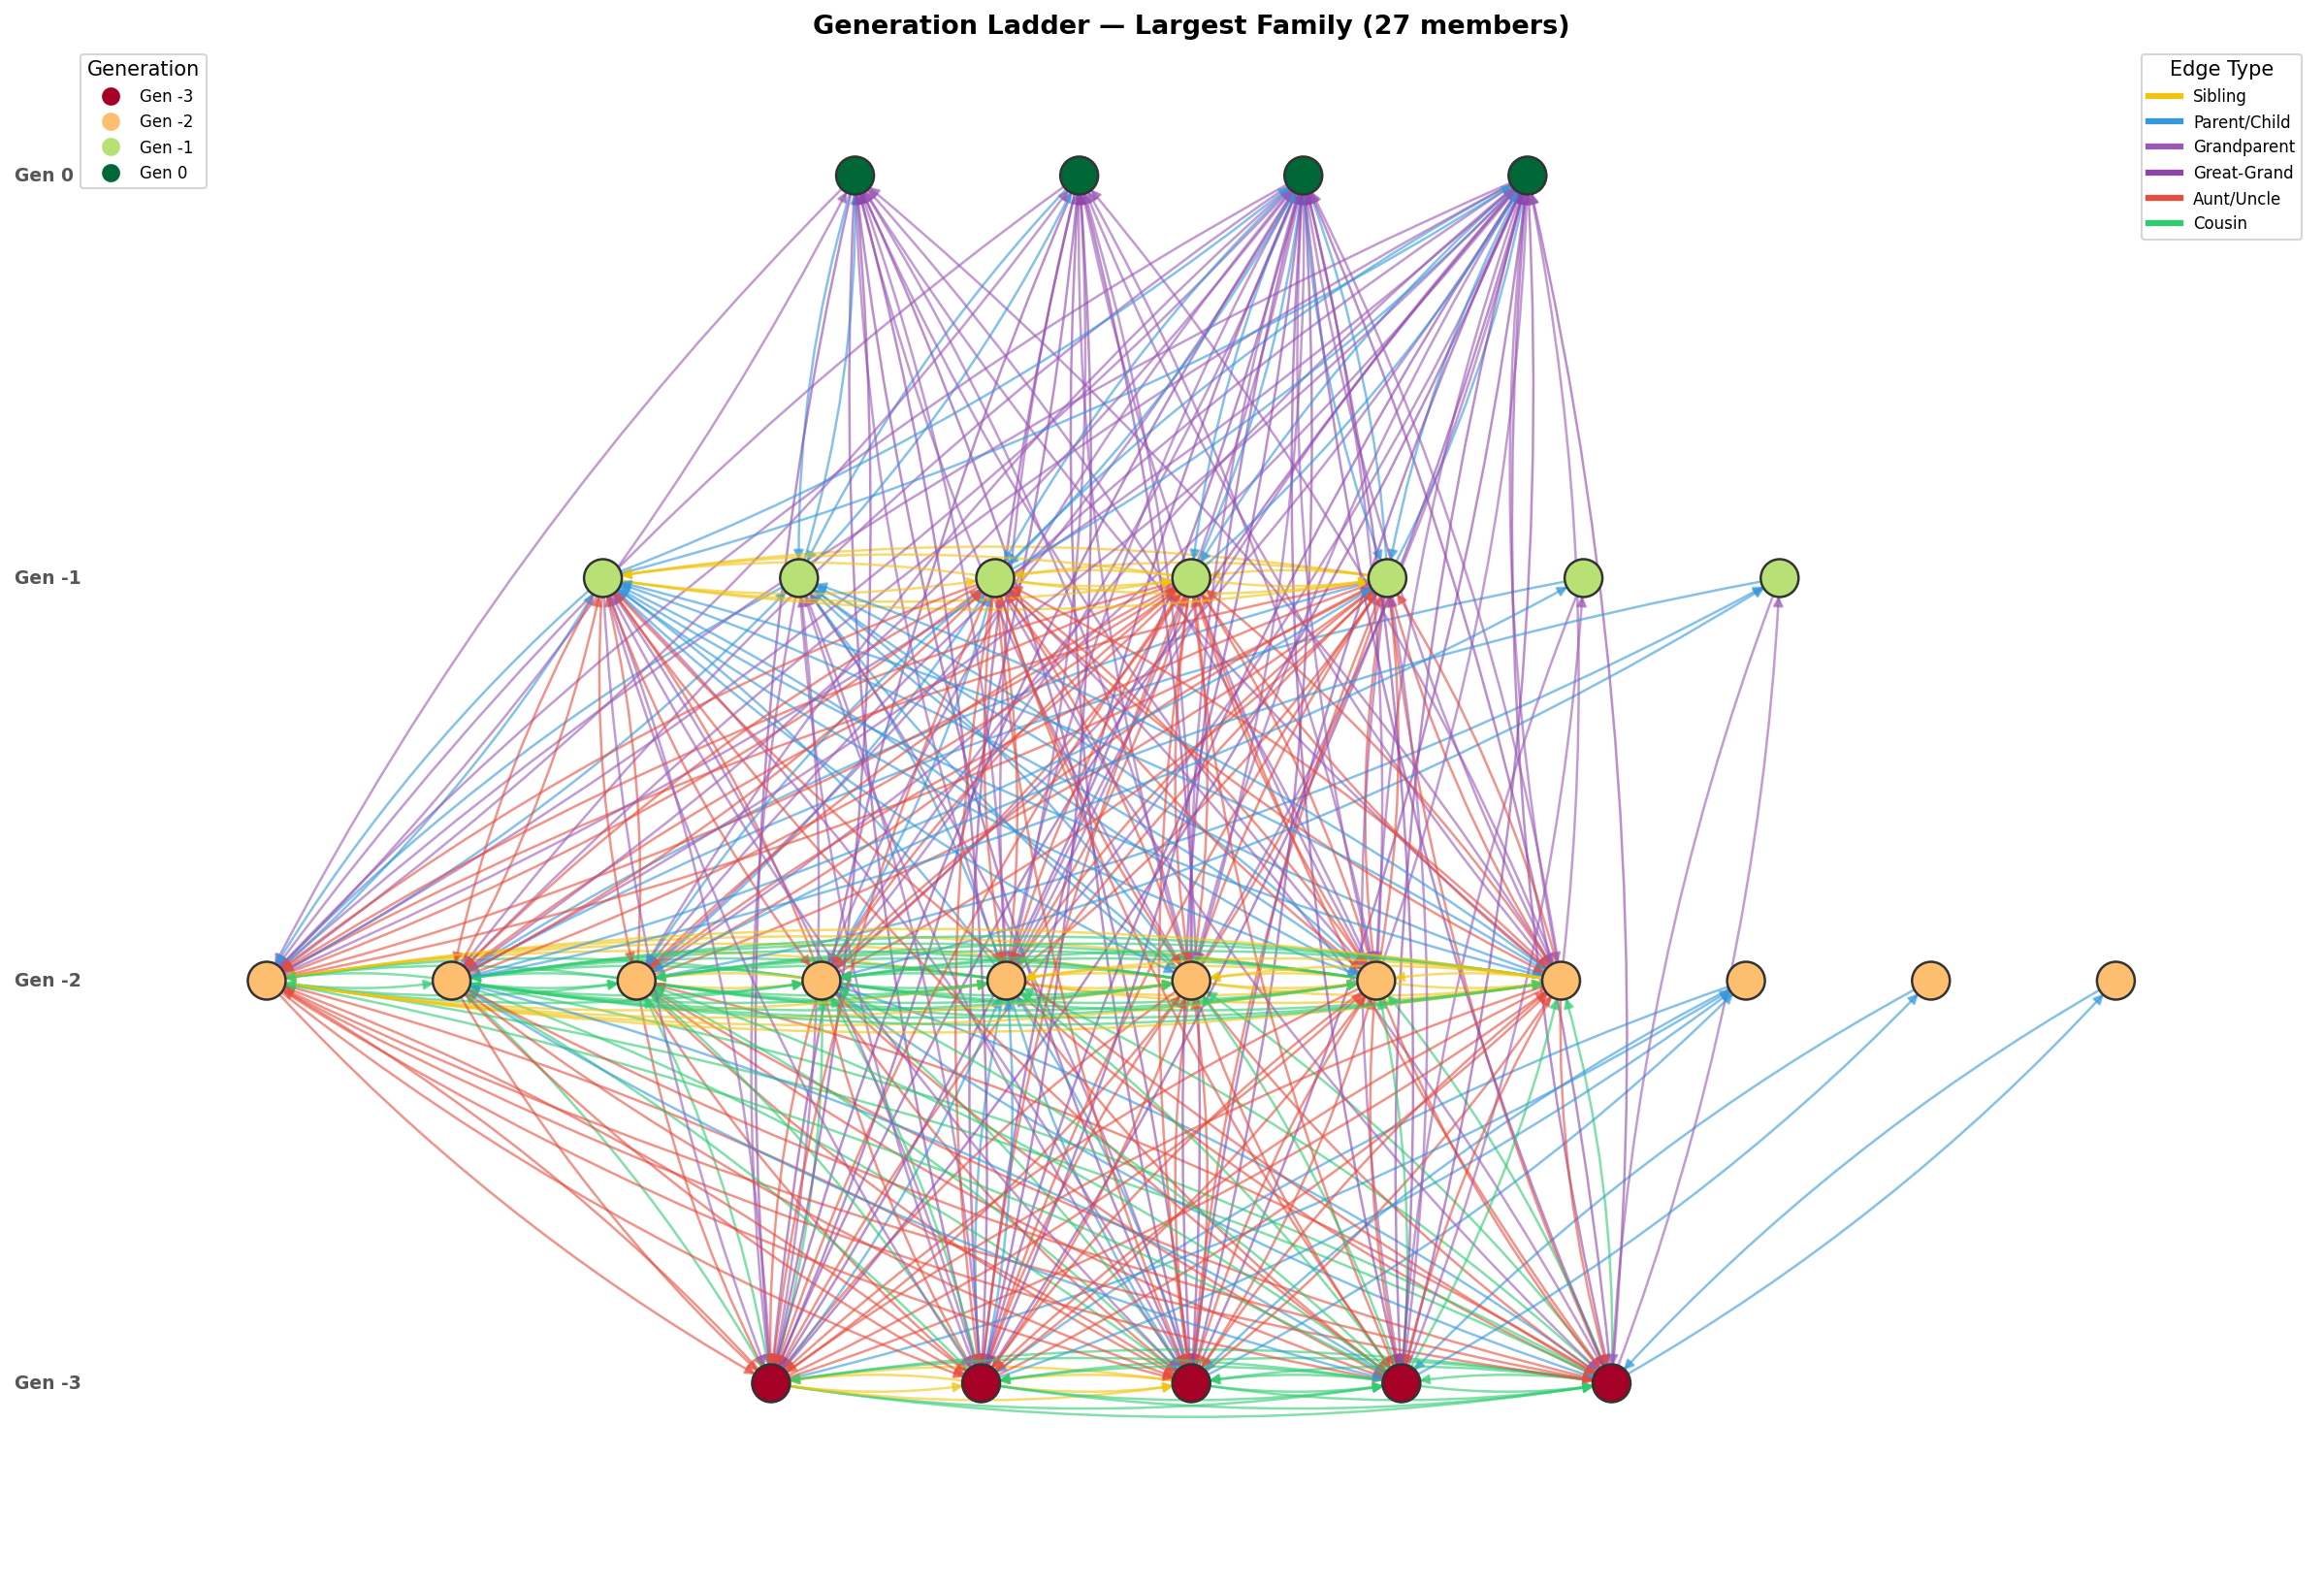
\includegraphics[width=0.85\textwidth]{task1/generation_ladder.png}
\caption{Generation ladder for the largest family: each row is one
generation, coloured red (oldest) to green (youngest). The wide middle
rows and narrow top/bottom rows reveal the demographic shape of the
family.}
\end{figure}

\begin{figure}[h]
\centering
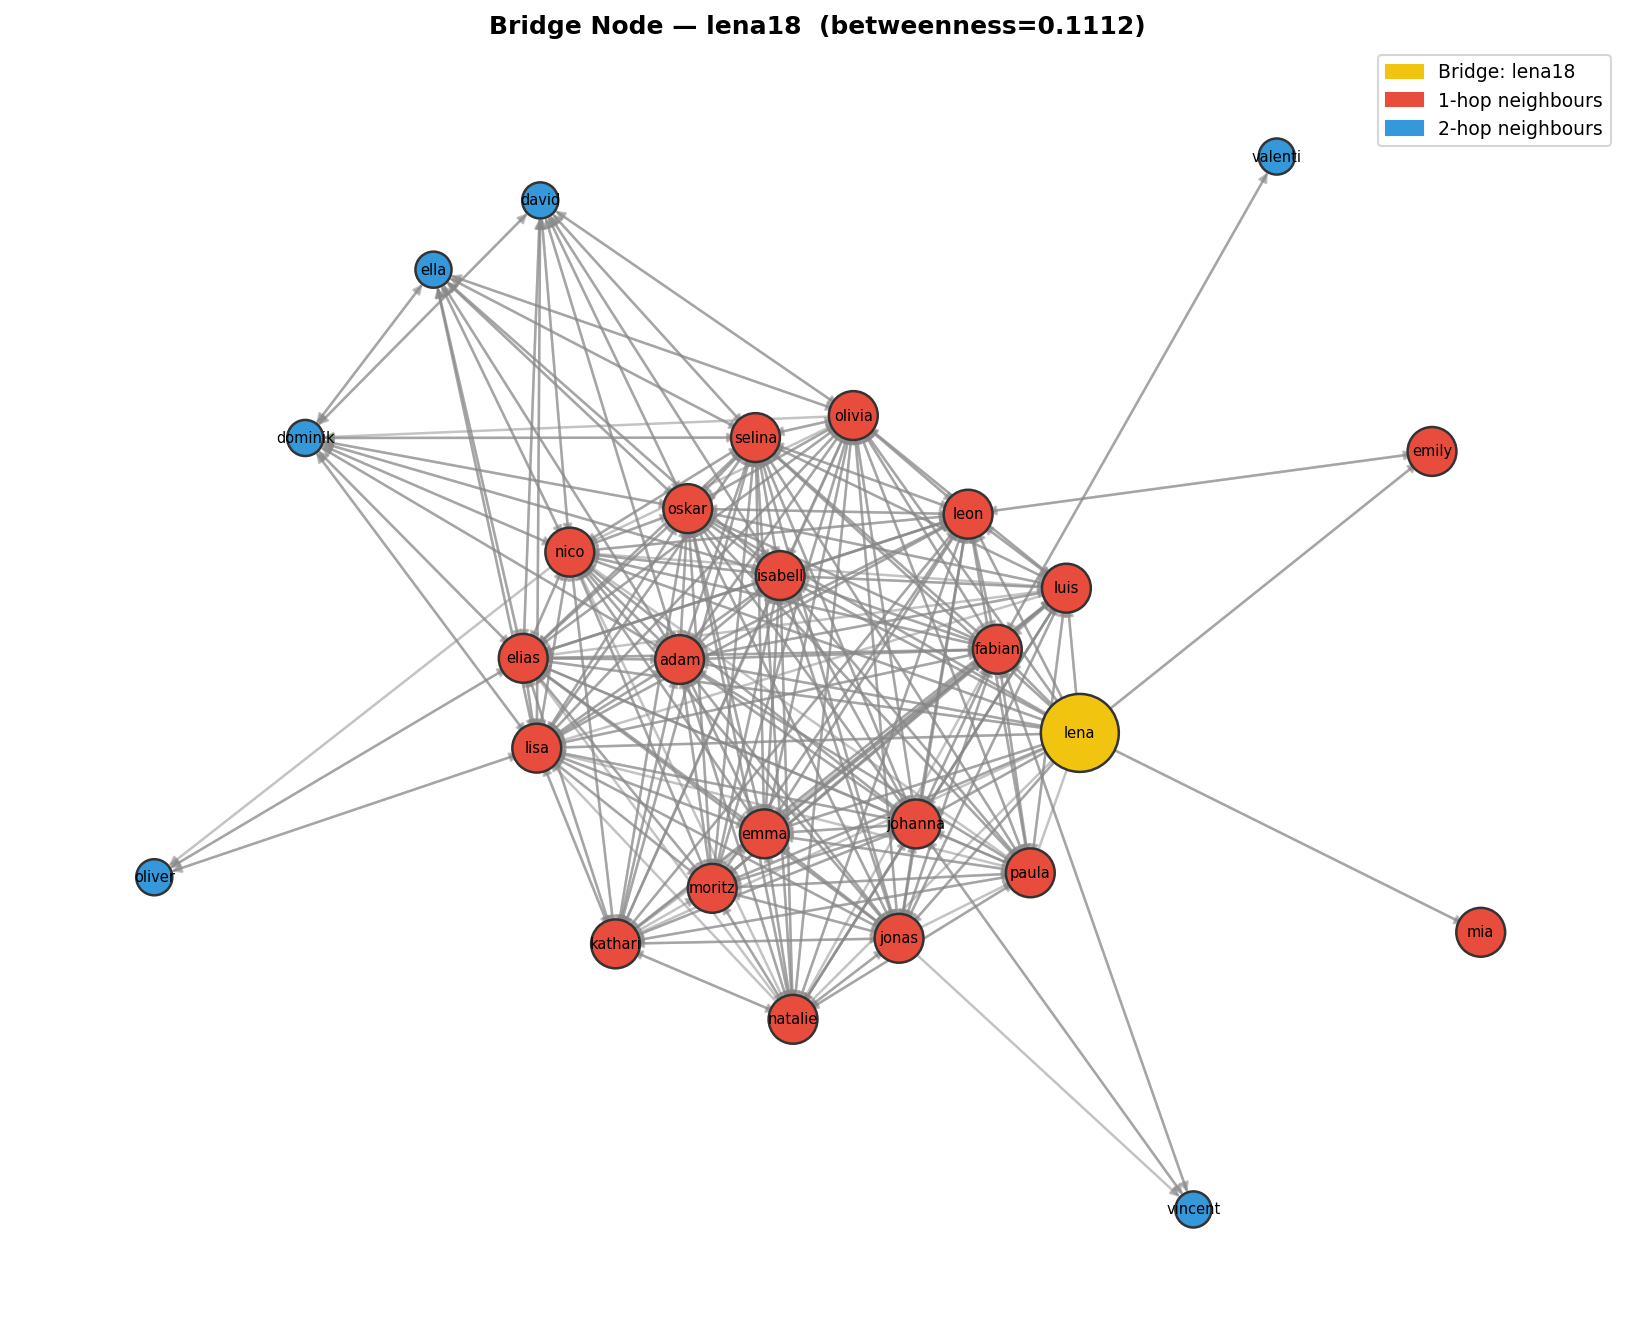
\includegraphics[width=0.7\textwidth]{task1/bridge_node.png}
\caption{Two-hop ego graph around the full graph's highest-betweenness
node --- the ``bridge'' individual connecting the most distinct branches.}
\end{figure}

\begin{figure}[h]
\centering
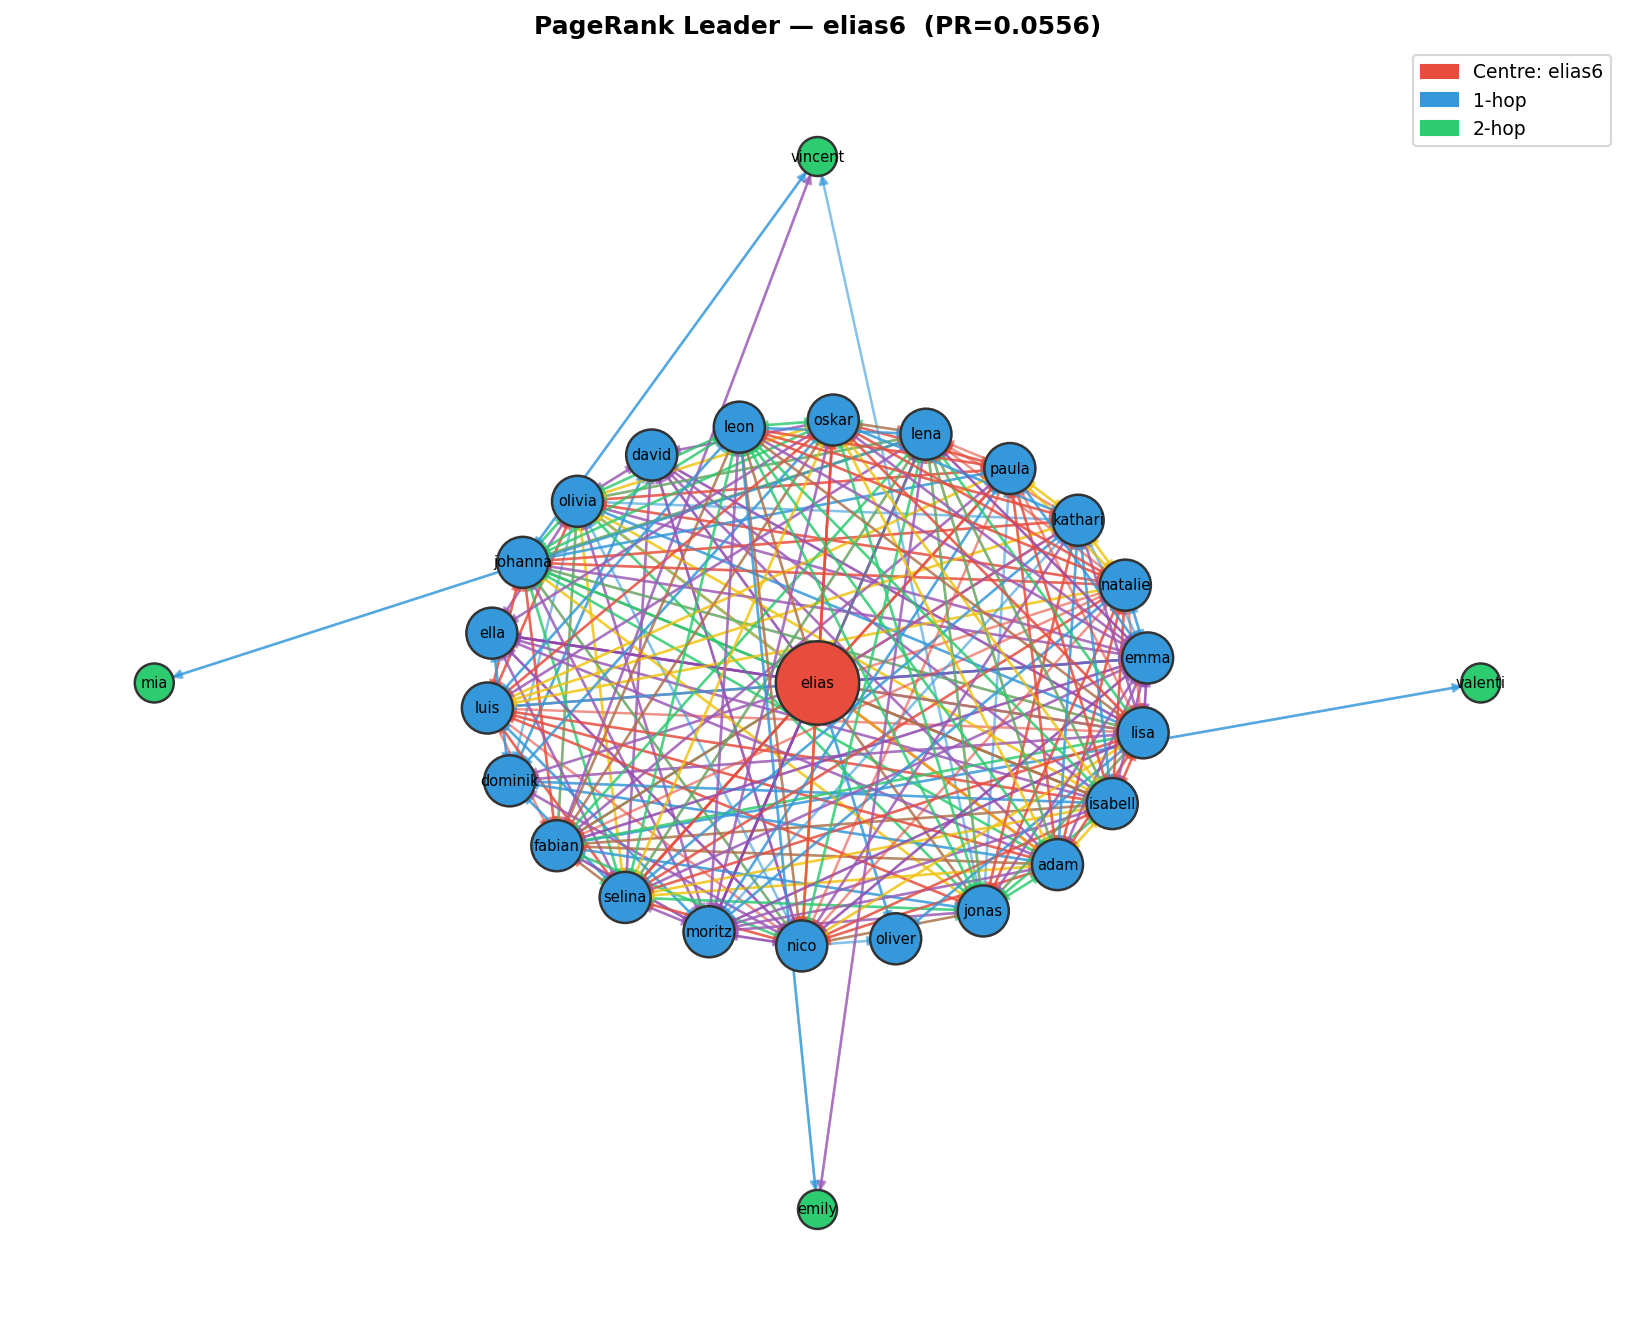
\includegraphics[width=0.7\textwidth]{task1/pagerank_ego.png}
\caption{Two-hop ego graph around the highest-PageRank node. The
star-like pattern of many descendants pointing toward the centre shows
recursive importance funnelling upward.}
\end{figure}

\section{Curiosity: Broker Stability Under Random Edge Deletion}

\subsection{Motivation}

Brokers were identified as key connectors. But is this metric reliable
under missing data? In real-world datasets, some relationships may go
unrecorded. If 20\% of the data is missing, does the same person remain
the top broker?

\subsection{Split Strategy}

Simulate data loss via random edge deletion, on the \emph{full} graph, at
$p = 10\%, 20\%, 30\%, 40\%, 50\%$; recompute global broker scores after
each deletion; compare against the original global top-10 and full
ranking. Because this runs on the full graph, the top-10 competes
globally across all 50 families, not within one.

\subsection{Evaluation Metrics}

\begin{itemize}[leftmargin=1.4em,itemsep=2pt]
\item \textbf{Jaccard similarity} of the top-10 sets: overlap between
      original and perturbed top-10.
\item \textbf{Spearman's $\rho$}: rank correlation across \emph{all}
      scored people, not just the top of the list.
\item \textbf{Survival rate}: fraction of the original top-10 still in
      the perturbed top-10.
\end{itemize}

\subsection{Results}

\begin{center}
\begin{tabular}{lcccc}
\toprule
\textbf{Drop \%} & \textbf{Jaccard (top-10)} & \textbf{Survival} & \textbf{Spearman $\rho$} & \textbf{Common $N$} \\
\midrule
10\% & $0.487 \pm 0.130$ & $0.645$ & $0.956$ & 1291 / 1306 \\
20\% & $0.389 \pm 0.164$ & $0.540$ & $0.924$ & 1276 / 1306 \\
30\% & $0.308 \pm 0.110$ & $0.460$ & $0.898$ & 1260 / 1306 \\
40\% & $0.200 \pm 0.081$ & $0.325$ & $0.867$ & 1241 / 1306 \\
50\% & $0.112 \pm 0.065$ & $0.195$ & $0.827$ & 1217 / 1306 \\
\bottomrule
\end{tabular}
\end{center}

\begin{figure}[h]
\centering
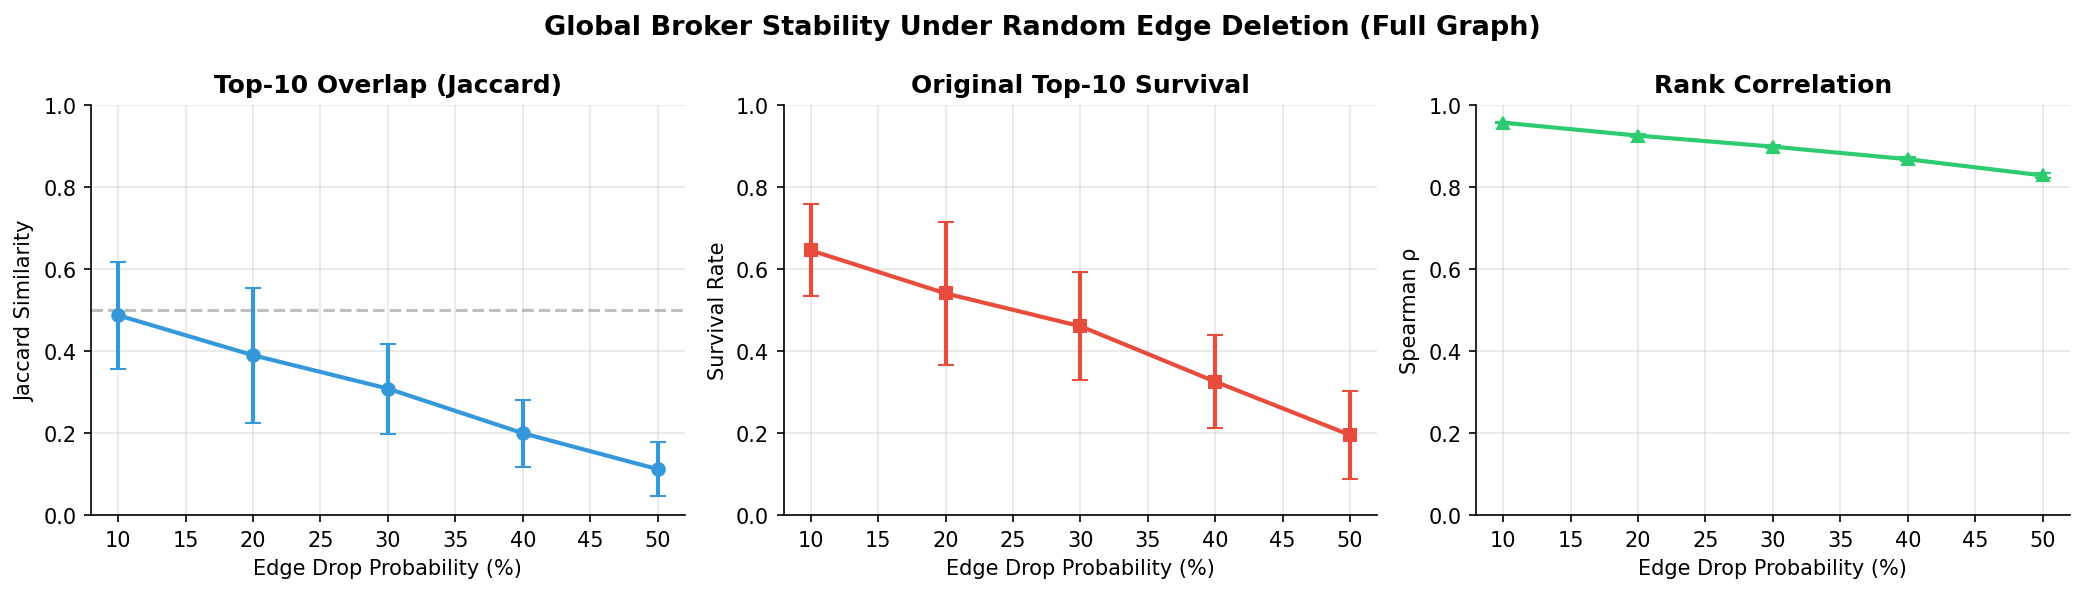
\includegraphics[width=0.95\textwidth]{task1/broker_stability.png}
\caption{Jaccard, survival, and Spearman $\rho$ as a function of edge
drop probability.}
\end{figure}

\subsection{Interpretation}

\textbf{Robustness:} at 50\% edge deletion, only about 20\% of the
original top-10 survive as top-10 --- the specific top ranking is
\emph{fragile}. \textbf{Rank preservation:} Spearman $\rho$ stays above
0.82 even at 50\% deletion --- the \emph{overall ordering} is far more
robust than the top-10 set. The reason both are true together: the top-10
are clustered within a narrow band of scores and are nearly tied, so
small perturbations reshuffle \emph{them} freely while the broad
separation between high- and low-scoring people persists.

\begin{why}
\textbf{A caveat worth stating precisely, not just the headline number.}
Broker Score excludes degree-$\leq 1$ nodes, and Spearman $\rho$ above is
computed only over people present in \emph{both} the original and
perturbed ranking (the ``Common $N$'' column). As more edges drop, more of
the most-damaged people fall below that degree threshold and leave the
comparison set entirely --- from 1{,}291 of 1{,}306 originally-scored
people at 10\% deletion down to 1{,}217 at 50\%. So part of the high
$\rho$ at heavy deletion is a \emph{survivorship artefact}: the people
hardest hit by the perturbation are quietly excluded from the very
correlation meant to measure how hard they were hit. This doesn't
overturn the conclusion --- rank order really is comparatively stable ---
but the honest version of the claim names the shrinking denominator
instead of hiding it.
\end{why}

\textbf{Conclusion:} brokers are structurally embedded, not accidental
artefacts of a few edges --- with the above caveat about what, precisely,
``robust'' is being measured over.

\section{Summary \& Key Findings}

\begin{itemize}[leftmargin=1.4em,itemsep=3pt]
\item \textbf{Disconnected structure:} 50 completely separate family
      trees with no cross-family edges.
\item \textbf{Degree inflation:} reciprocal relations inflate directed
      degree counts relative to family size.
\item \textbf{Generational dominance:} middle generations act as
      structural glue across every centrality metric.
\item \textbf{High clustering, low density, simultaneously:} extended
      kinship ties make clustering high \emph{within} families; the fact
      that families never touch \emph{each other} makes global density
      low. Neither implies the graph is ``tree-like.''
\item \textbf{Robustness, with a caveat:} key figures remain broadly
      identifiable even under severe simulated data loss (50\% edges
      dropped), though part of that apparent robustness is a
      survivorship artefact in how the comparison set is defined (\S7.5).
\end{itemize}

% ================================================================== TASK 2
\starttask{Task 2 --- Community Detection}

\section{Introduction}

This task answers three questions:

\begin{enumerate}[leftmargin=1.6em,itemsep=2pt]
\item \textbf{Global detection:} can standard algorithms recover the 50
      distinct families?
\item \textbf{Local structure:} how do we detect sub-communities within
      large families?
\item \textbf{Metrics:} can we give a new metric for measuring
      relatedness?
\end{enumerate}

\section{Graph Construction Strategy}

To make community-detection algorithms understand a family KG, I built
two different weighted, undirected versions of the graph.

\subsection{The ``Generation Gap'' graph (\texorpdfstring{$G_{\text{gen}}$}{G\_gen})}

Edge weight derived from the generation weights of \S2.2 in Task 1
(father is $+1$, etc.).

\begin{why}
\textbf{A modelling bug, not a typo, and worth explaining rather than
quietly patching.} The natural first idea is to weight an edge by
$|\text{generation gap}|$: parent--child $= 1$, grandparent $= 2$,
siblings and cousins $= 0$ (same generation). But Louvain and Leiden are
run with \texttt{weight='weight'}, and a zero-weight edge contributes
\emph{nothing} to modularity --- it is, for the algorithm's purposes,
not there. That silently deletes every sibling and same-generation-cousin
tie from $G_{\text{gen}}$, arguably the strongest ties in the graph.

The fix is to convert the generation gap to a \emph{similarity} before
using it as a weight: $w = 1/(1+|\text{gap}|)$, so siblings $\to 1.00$,
parent/child $\to 0.50$, grandparent $\to 0.33$, and so on --- monotonic
in the same direction as before, but never zero.
\end{why}

\subsection{The ``Closeness Survey'' graph (\texorpdfstring{$G_{\text{close}}$}{G\_close})}

The goal here is to measure emotional closeness. I used weights inspired
by sociological studies on \emph{intergenerational solidarity} (Bengtson
\& Roberts, 1991; Dykstra \& Fokkema, 2011).

Why bother with a second graph at all: under plain generation weights, a
``second cousin'' and a ``sibling'' are both 1 edge, 0 generations away
--- identical. But a sibling is significantly ``closer.'' This graph is
designed to fix exactly that (and is also what \S7's WRD metric is built
from).

The weights (high = close): 10/10 for parent $\leftrightarrow$ child,
9/10 for siblings, and so on down to 2/10 for second cousins (full table
in the notebook).

\section{Modularity-Based Algorithms}

\subsection{What is modularity?}

Modularity ($Q$) measures how much more densely connected a community is
than you would expect by chance, given the same degree distribution.

\subsection{The Louvain Algorithm}

A greedy algorithm: for each person, ask ``if I move you to a neighbour's
community, does $Q$ go up?'', repeat until $Q$ stops improving.
\textbf{Result:} perfect recovery of all 50 families. Since the families
are disconnected, the algorithm finds the cuts trivially.

\subsection{The Leiden Algorithm}

An improved Louvain: Louvain can produce a community that is technically
``one community'' but is actually two barely-connected chunks; Leiden
adds a refinement step guaranteeing every community is internally
connected. At low resolution it perfectly finds the 50 families (same as
Louvain); at high resolution it starts splitting families into
sub-communities (nuclear households). As resolution increases past 1.0,
the algorithm shifts from finding ``whole families'' to finding
``nuclear households.''

\begin{figure}[h]
\centering
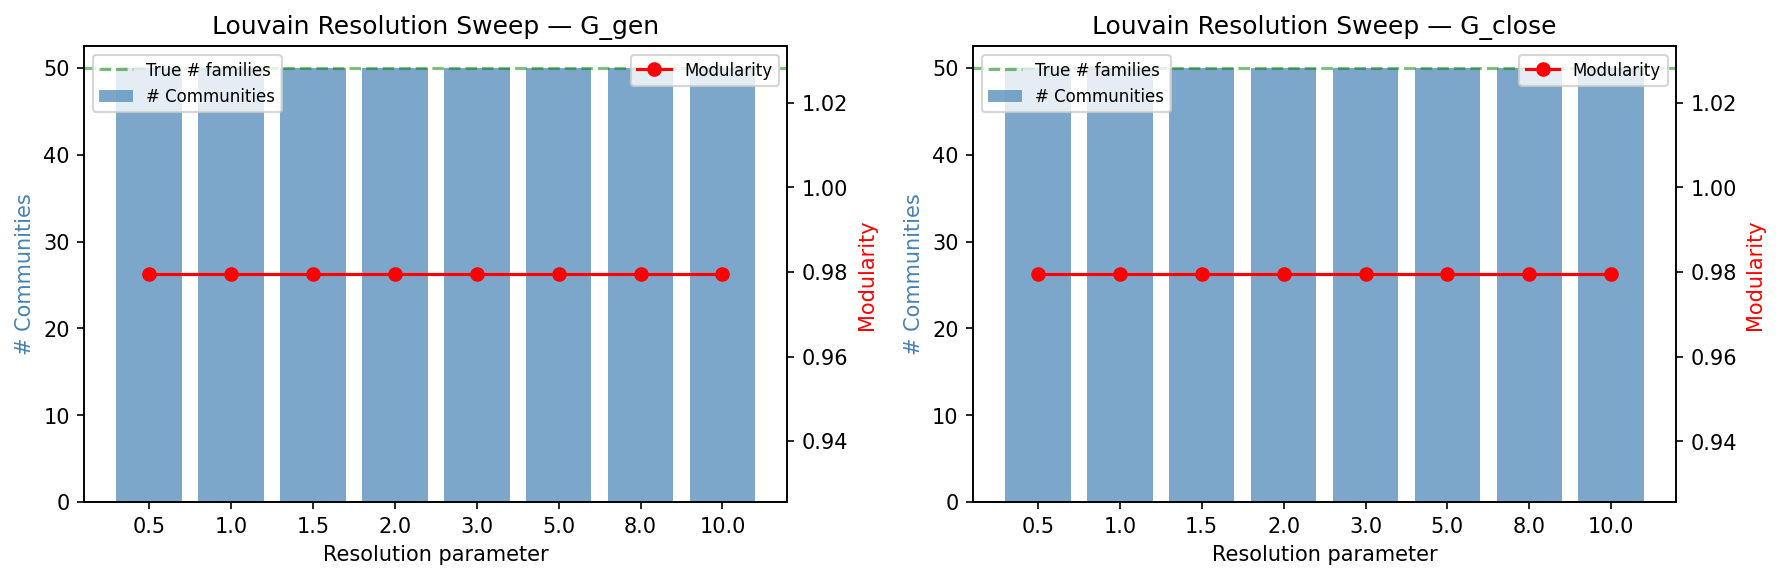
\includegraphics[width=0.92\textwidth]{task2/louvain_resolution_sweep.png}
\caption{Louvain community count and modularity as resolution increases,
for both graph weightings.}
\end{figure}

\begin{figure}[h]
\centering
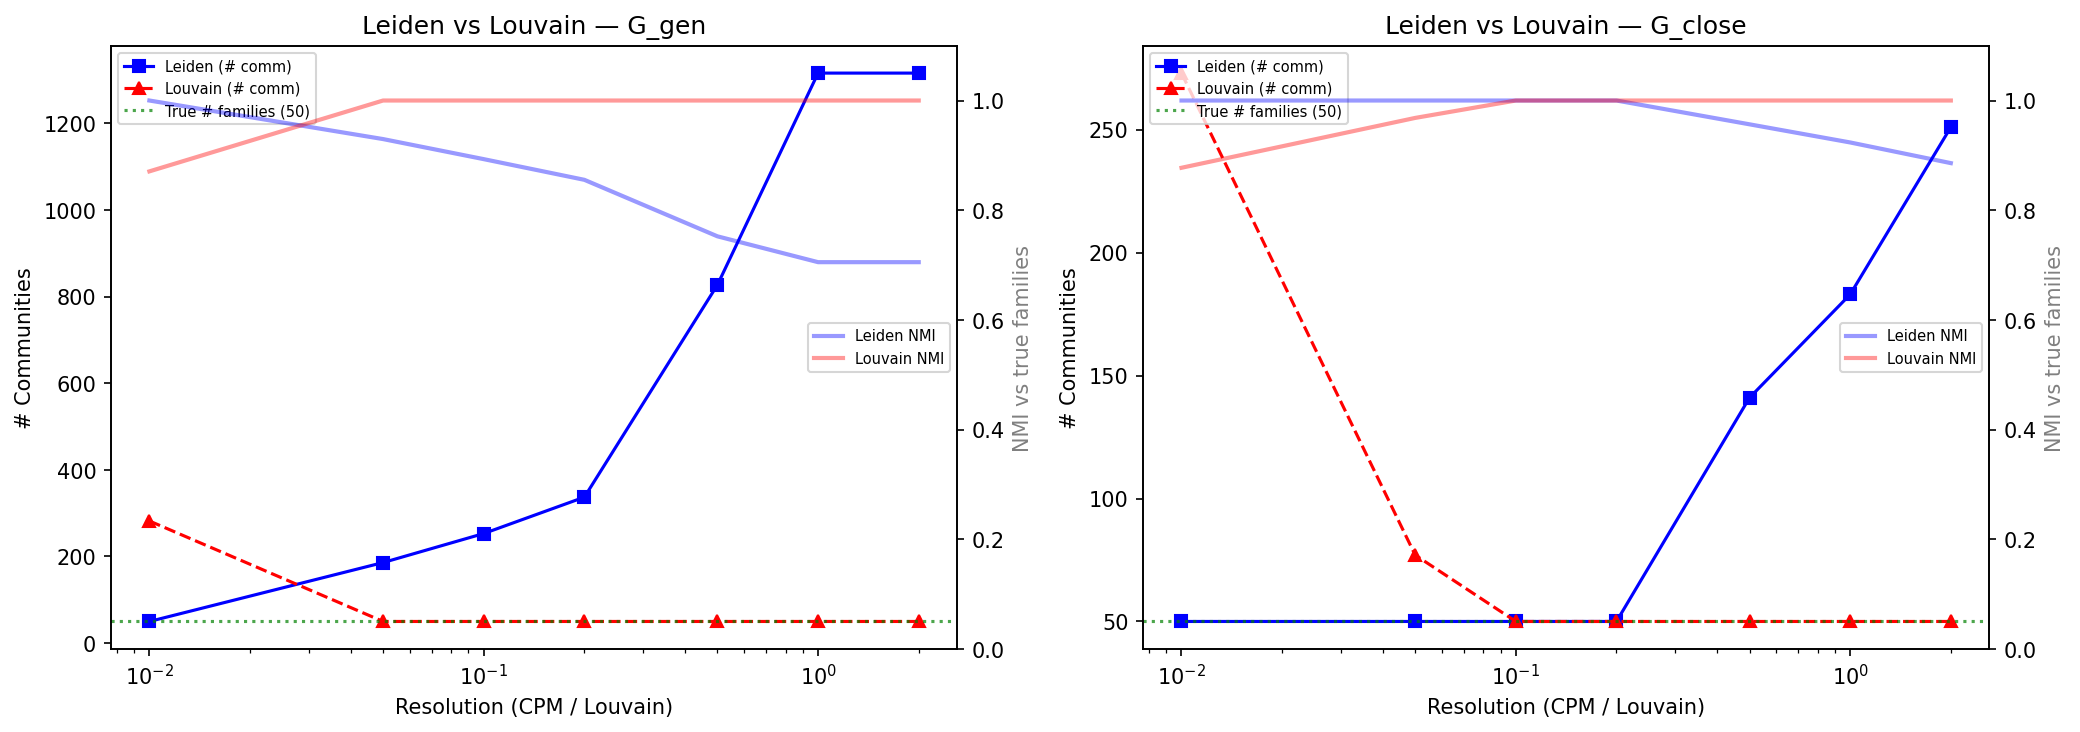
\includegraphics[width=0.92\textwidth]{task2/leiden_vs_louvain_sweep.png}
\caption{Leiden vs.\ Louvain agreement (NMI) and community count across a
CPM resolution sweep. They agree at family-level detection and may
diverge on sub-family splits.}
\end{figure}

\section{Girvan--Newman (Divisive Clustering)}

\subsection{How it works}

Compute edge-betweenness centrality for every edge, remove the edge with
the highest betweenness, recompute, repeat. At each step the number of
connected components grows, giving a hierarchy. Cost is roughly
$O(m^2 n)$ --- expensive.

\subsection{Findings}

\textbf{Family level: not run, and deliberately so.} Girvan--Newman
removes the highest-betweenness edge repeatedly; since no edge bridges
two families, \emph{no edges need to be removed at all} before the graph
already has 50 connected components matching the ground truth. An earlier
draft of this analysis ran a version of this ``recovery'' by building a
partition directly from the known components and then comparing that
partition to itself, which scores a perfect NMI/ARI $= 1.0$ by
construction --- a tautology, not a measurement, and it has been removed
from the comparison table in \S6 for exactly that reason. The reasoning
above is what the (unrun) full-graph result would show, and it doesn't
need a run to justify.

\textbf{Sub-family level:} inside a single family, everyone is highly
connected to everyone else (parents, grandparents, cousins); there are no
clean ``bridges'' to cut. Girvan--Newman's best-modularity split on the
largest family reaches $Q \leq 0$ for the closeness-weighted graph ---
\emph{worse than a random split}, i.e.\ genuinely no meaningful
sub-structure by this method, not merely a weak one. I report it as
``best-modularity split (still $\leq 0$)'' rather than ``optimal,''
because ``optimal'' implies the split is good, and a non-positive
modularity is precisely the algorithm failing to find any real
structure. Because \texttt{girvan\_newman} ignores edge weights entirely,
the split itself is identical for the generation-weighted and
closeness-weighted graphs; only the reported modularity \emph{value}
(which does use the weights) differs between the two.

\begin{figure}[h]
\centering
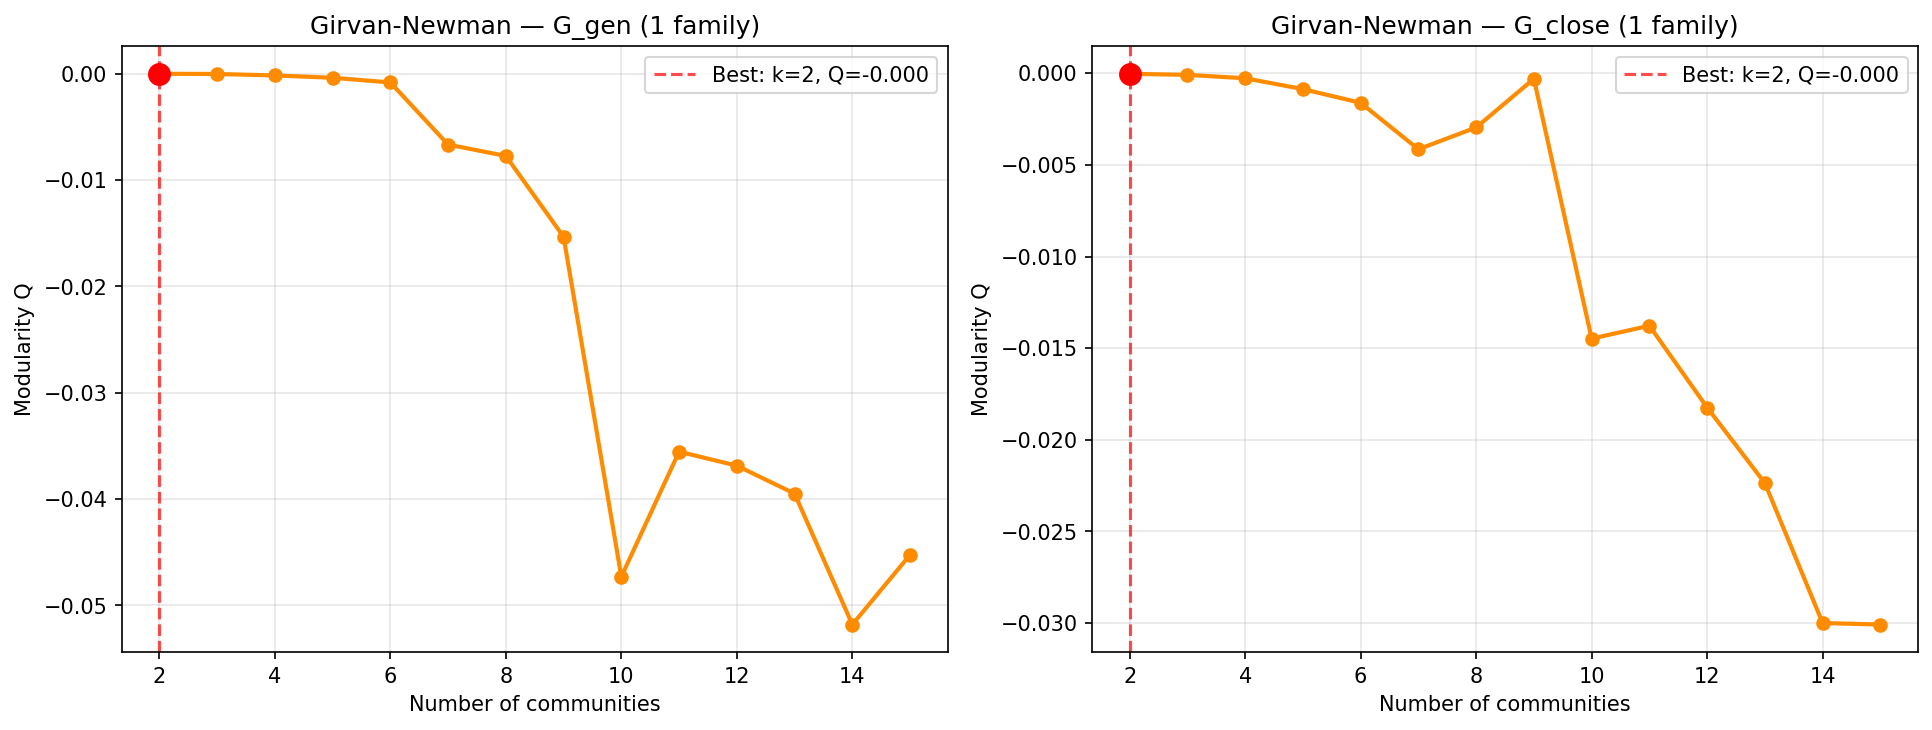
\includegraphics[width=0.92\textwidth]{task2/girvan_newman_modularity.png}
\caption{Modularity vs.\ number of sub-communities as Girvan--Newman
splits the largest family. The best-modularity point is marked --- note it
sits at or below $Q=0$.}
\end{figure}

\begin{figure}[h]
\centering
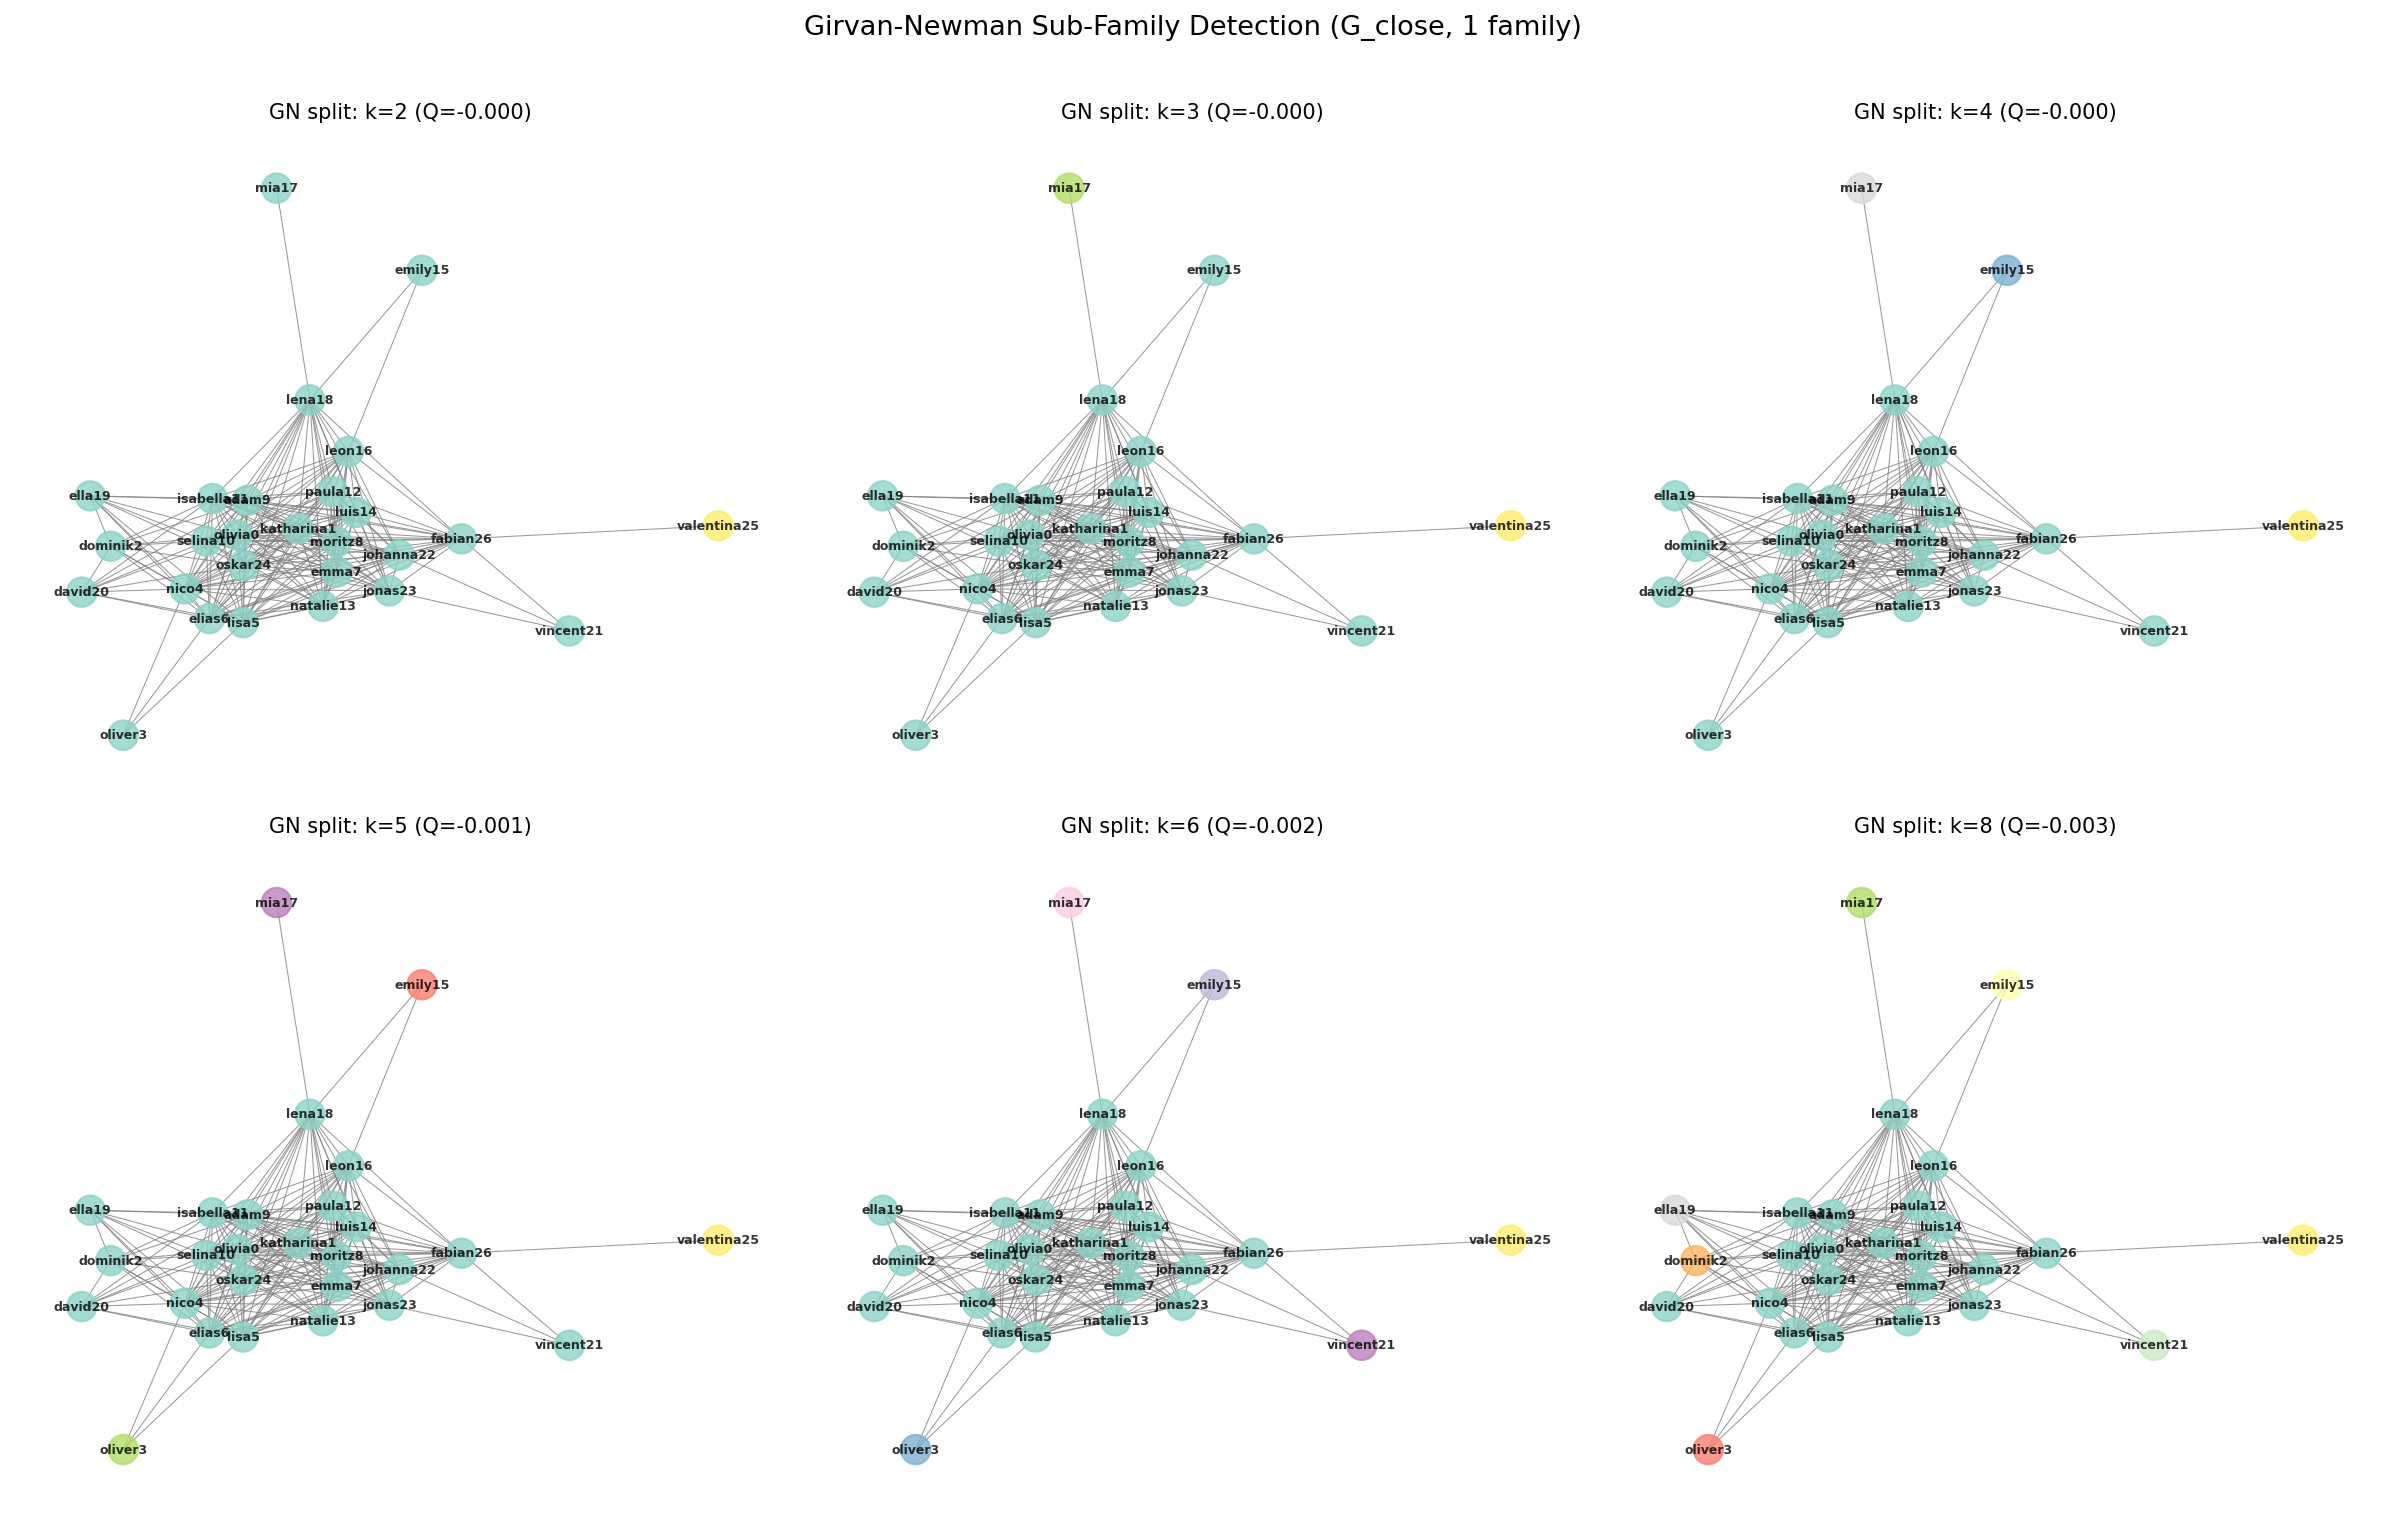
\includegraphics[width=0.92\textwidth]{task2/girvan_newman_splits.png}
\caption{Girvan--Newman splitting one family into increasing numbers of
pieces. Modularity stays low throughout, confirming that dense
extended-family subgraphs have no clean internal bridges to cut.}
\end{figure}

\section{Machine Learning: Node2Vec + KMeans}

\subsection{Concept}

Instead of looking at edges explicitly, use learned embeddings. Take
biased random walks over the graph; if two people co-occur often in the
same walk, treat them as similar (the Word2Vec idea, transplanted to
graphs); map every person to a vector and cluster with KMeans.

\subsection{Findings}

\textbf{Family separation:} perfect --- the embedding cloud for one
family sits far from every other family's cloud. \textbf{Provably
irrelevant knobs:} sweeping the walk parameters $p,q$ across
$(1,0.5),(1,2),(0.5,1),(2,1),(0.25,4)$ gives NMI $=1.0$ every single time,
because a random walk on a disconnected graph can never leave the
component it started in --- the parameters have nothing to act on.
\textbf{Local structure:} within one family, Node2Vec + KMeans (with an
elbow/silhouette scan) finds a small number of sub-groups that broadly
align with generation.

\begin{figure}[h]
\centering
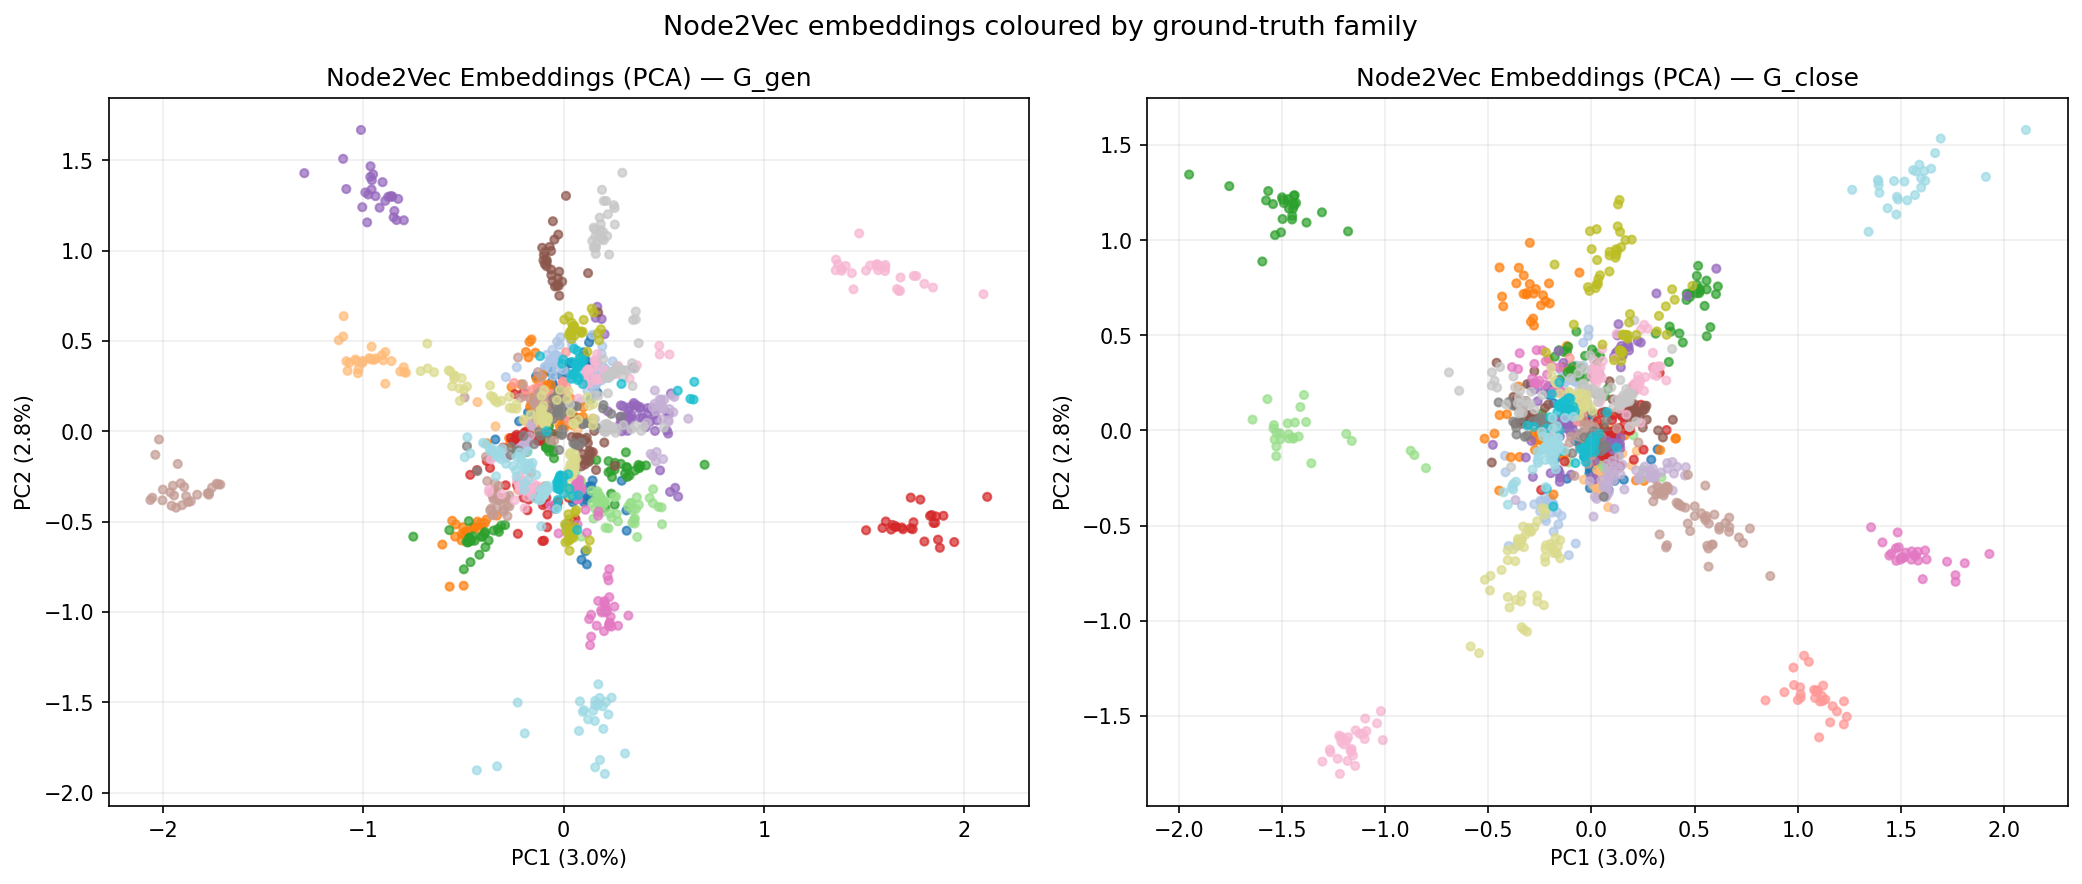
\includegraphics[width=0.92\textwidth]{task2/node2vec_pca.png}
\caption{Node2Vec embeddings (PCA to 2D), coloured by ground-truth
family. Total separation --- learned purely from graph structure, no
labels involved.}
\end{figure}

\begin{figure}[h]
\centering
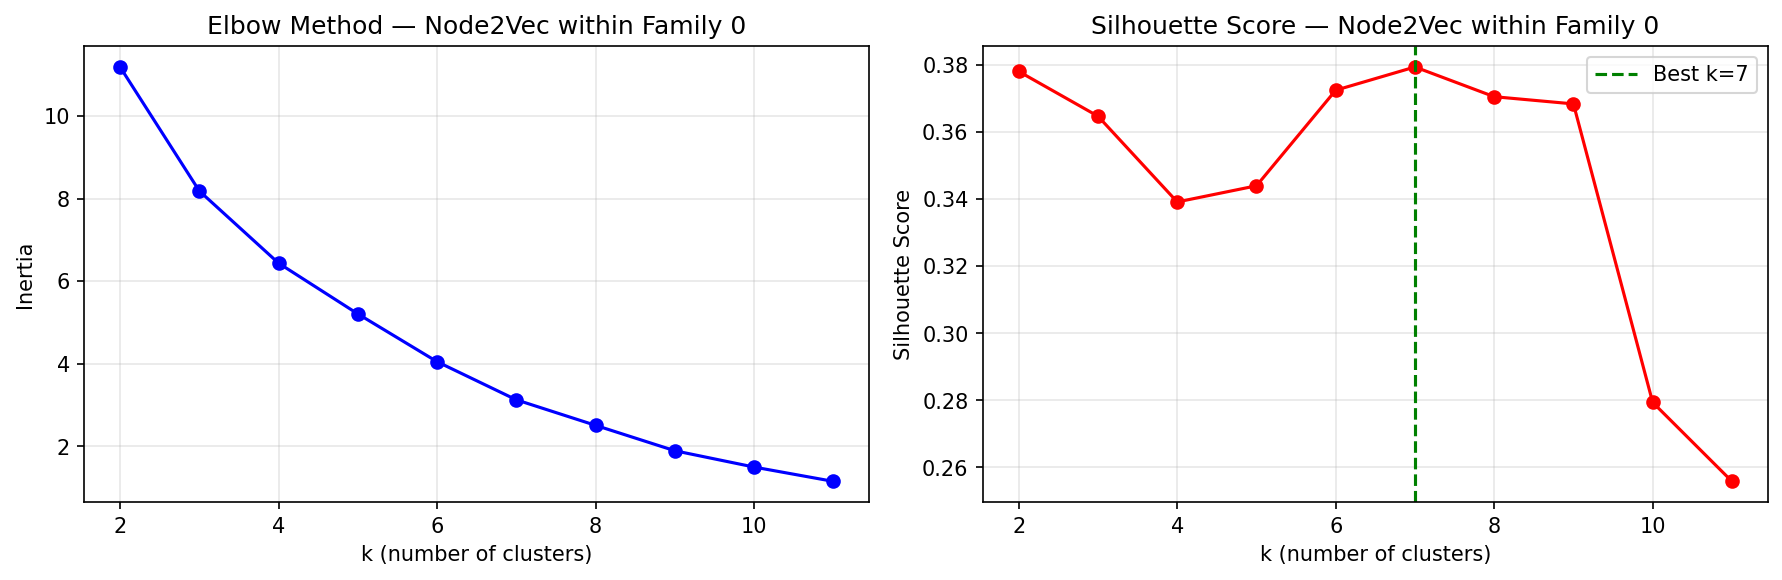
\includegraphics[width=0.85\textwidth]{task2/node2vec_subfamily_elbow.png}
\caption{Elbow (inertia) and silhouette score for KMeans on Node2Vec
embeddings restricted to one family, used to pick the sub-cluster count.}
\end{figure}

\section{Comprehensive Comparison}

\subsection{Summary Table}

\begin{center}
\begin{tabular}{lccc}
\toprule
\textbf{Method} & \textbf{Communities found} & \textbf{Modularity} & \textbf{NMI / ARI} \\
\midrule
Louvain & 50 & 0.979 & 1.00 / 1.00 \\
Leiden & 50 & 0.979 & 1.00 / 1.00 \\
Node2Vec + KMeans & 50 & 0.979 & 1.00 / 1.00 \\
\bottomrule
\end{tabular}
\end{center}

Girvan--Newman is intentionally absent from this table (\S4.2): a
tautological row --- comparing the known components to themselves ---
used to sit here scoring a guaranteed 1.0, and it has been removed rather
than kept for the sake of having four rows.

\begin{figure}[h]
\centering
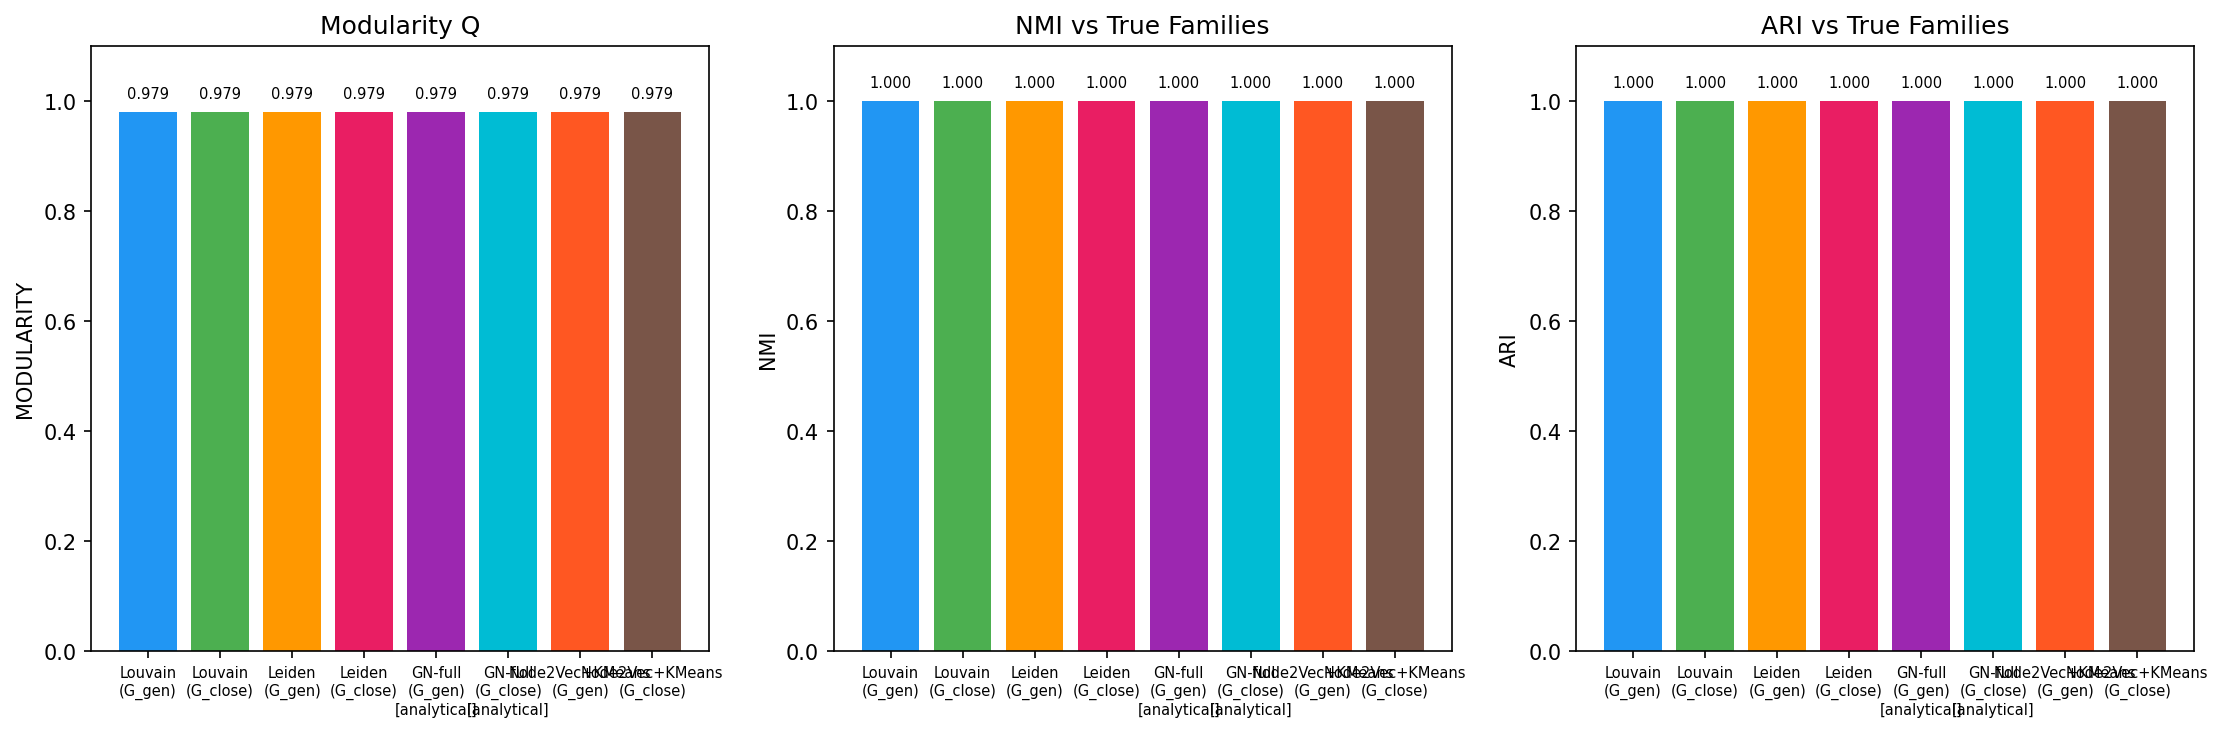
\includegraphics[width=0.85\textwidth]{task2/community_comparison.png}
\caption{Modularity, NMI, and ARI for the three family-level methods
actually run. All three achieve near-perfect scores, as expected for 50
disconnected components.}
\end{figure}

All three achieve near-perfect scores, which is not by itself an
impressive result and is not treated as one: the families are
disconnected components, so any connectivity-aware method separates them
trivially. The real value of Task 2 is in what follows.

\subsection{Sub-Community Deep Dive}

Forcing the algorithms to look deeper (Leiden CPM, resolution 0.5, on
$G_{\text{close}}$) splits the 50 families into 141 sub-communities
(average 2.8 per family), which fall into a few recognisable shapes:

\begin{itemize}[leftmargin=1.4em,itemsep=3pt]
\item \textbf{Core groups} (roughly 15--25 people): the densely
      interlinked bulk of a family.
\item \textbf{Singletons:} 78 of 141 sub-communities (55\%) are exactly
      one person. Investigating why: these people average about 1 edge
      inside the family versus about 12 for everyone else. They are
      isolated because of \emph{low degree}, not weak relationships ---
      CPM requires a node's internal edge density to clear a threshold,
      and one edge cannot clear it. This is a data-sparsity artefact of
      how these particular people happen to be connected, not a
      sociological finding about them.
\item \textbf{Nuclear-family-shaped units,} where the data actually
      supports the label. One case-study sub-community of 4 people has
      exactly 2 members in the oldest generation and 2 in the next, held
      together by 8 parent--child edges and 2 sibling edges --- I check
      this shape explicitly (oldest-generation count, generation span)
      rather than asserting every small sub-community is a ``nuclear
      family,'' since not all of them are.
\end{itemize}

\begin{figure}[h]
\centering
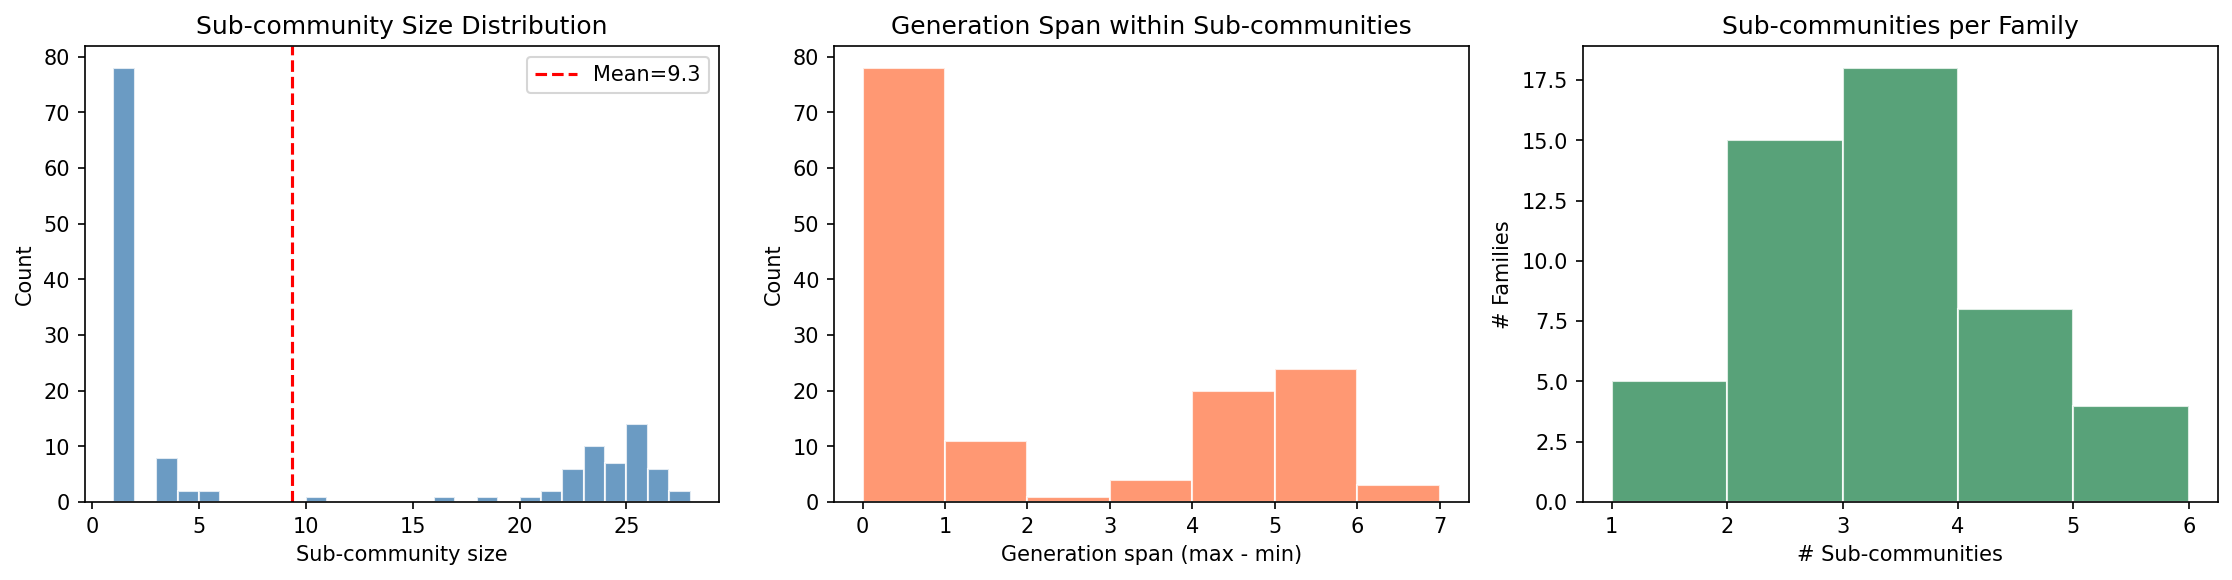
\includegraphics[width=0.92\textwidth]{task2/subfamily_analysis.png}
\caption{Distribution of sub-community sizes (note the large singleton
spike), generation span within sub-communities, and sub-communities per
family.}
\end{figure}

A larger case-study sub-community (24 of 26 members of one family, 6
generations) is better described as an \emph{extended-family backbone} ---
multiple nuclear units linked through parent/grandparent/aunt/uncle ties,
not a single household. The 2 missing members are peripheral relatives
with weaker ties to this core; MetaFam has no in-law relations at all, so
that specific explanation for ``who's missing'' can be ruled out rather
than guessed at.

\section{Weighted Relationship Distance (WRD)}

Standard graph metrics fail for genealogy: plain hop count says a sibling
and a second cousin are both ``1 hop away,'' which is obviously wrong.

\subsection{The metric}

\[
\mathrm{WRD}(u,v) \;=\; \min_{\text{paths } P:\, u \to v} \;
\sum_{(i,j)\in P} \frac{1}{\mathrm{closeness}(r_{ij})}
\]

Invert the closeness score so it becomes a \emph{cost}: parent
(closeness 10) $\to$ cost 0.1 (cheap to cross, i.e.\ ``close''); second
cousin (closeness 2) $\to$ cost 0.5 (expensive, i.e.\ ``far''). WRD
between two people is the \emph{cheapest total path} between them,
computed with a standard shortest-path algorithm (Dijkstra) --- not just
the cost of a single labelled edge. The minimisation over paths is the
entire point: it lets a cheaper multi-hop route through closer
intermediaries beat an expensive direct edge, which is exactly what
happens in practice (see the second-cousin row below).

\begin{center}
\begin{tabular}{llcc}
\toprule
\textbf{Pair} & \textbf{Relation} & \textbf{Hops} & \textbf{WRD} \\
\midrule
olivia0 -- lisa5 & \rel{motherOf} & 1 & 0.100 \\
olivia0 -- selina10 & \rel{sisterOf} & 1 & 0.111 \\
katharina1 -- nico4 & \rel{grandmotherOf} & 1 & 0.143 \\
katharina1 -- leon16 & \rel{auntOf} & 1 & 0.167 \\
olivia0 -- leon16 & \rel{girlCousinOf} & 1 & 0.200 \\
lena18 -- fabian26 & \rel{girlSecondCousinOf} & 1 & 0.393 \\
\bottomrule
\end{tabular}
\end{center}

Six pairs, all at hop count 1, correctly spread across a range. The last
row is the interesting one: a \emph{direct} \rel{girlSecondCousinOf} edge
would cost $1/2 = 0.500$, but this specific pair's shortest WRD path is
only $0.393$ --- WRD found a cheaper route through closer intermediaries.
That is the metric working exactly as designed, not a discrepancy to
explain away.

\begin{why}
\textbf{Where the closeness numbers came from, and the honest caveat.}
They are grounded in the intergenerational-solidarity literature from
family sociology (Bengtson \& Roberts, 1991; Dykstra \& Fokkema, 2011),
which measures family cohesion along affectual (emotional), associational
(contact frequency), and functional (mutual support) dimensions. The
weights here operationalise the affectual dimension. The caveat: these
are still \emph{hand-set numbers reflecting one cultural model of
kinship}, not learned or independently validated. In a culture with
different family structures they would plausibly be different. The
metric's \emph{form} --- reciprocal-cost shortest path --- is the
contribution; the specific constants are a defensible but replaceable
choice.
\end{why}

\begin{figure}[h]
\centering
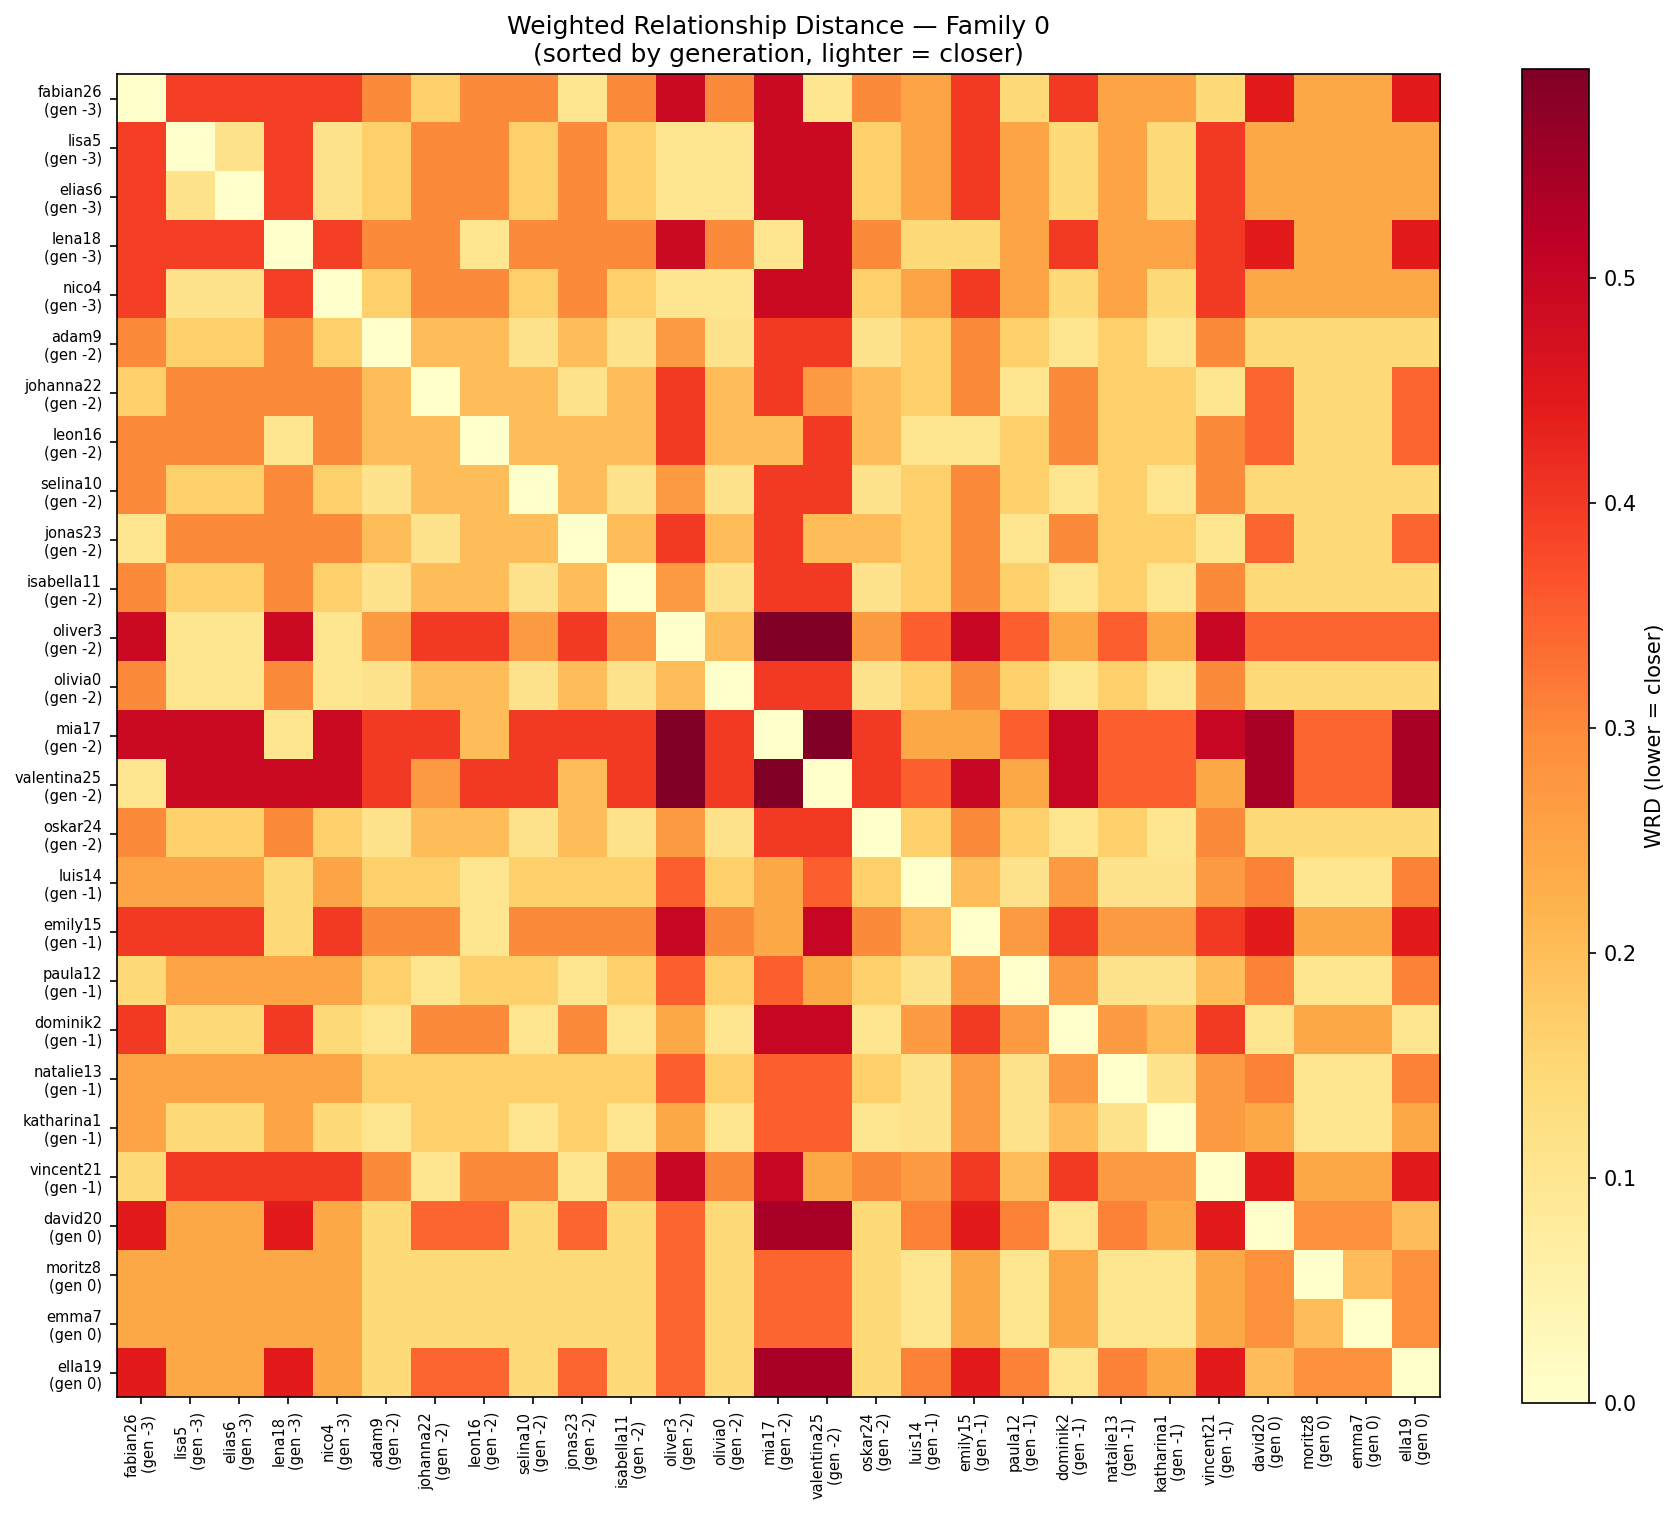
\includegraphics[width=0.62\textwidth]{task2/wrd_heatmap.png}
\caption{WRD between every pair in one family, sorted by generation.
Lighter = closer. The block structure is generational: same-generation
pairs are light, cross-generation pairs darken as the gap widens.}
\end{figure}

\section{Hierarchical Clustering Analysis}

I compared two ways of viewing a family: \textbf{Leiden} (density) groups
people who are densely inter-connected --- the social-clique reading.
\textbf{WRD} (distance) groups people who are closely related by the
shortest-path metric above --- the family-tree-branch reading.

\subsection{Method note: average-linkage, not Ward}

Feeding the WRD distance matrix into hierarchical clustering requires
picking a linkage rule. WRD distances are shortest-path costs, not
coordinates in a Euclidean space, so I use \textbf{average-linkage}
rather than Ward's method: Ward's objective is to minimise
within-cluster \emph{variance}, which assumes a Euclidean geometry that a
shortest-path metric does not have. \texttt{scipy} will run Ward on any
distance matrix regardless, but the result then does not mean what
Ward's stated objective claims it means. Average-linkage --- merge the
pair of clusters whose \emph{average} pairwise distance is smallest --- is
valid for an arbitrary metric, so the comparison below rests on a
defensible method rather than a technically-runnable-but-inapplicable
one.

\subsection{Findings}

Agreement between WRD-average-linkage and Leiden CPM is low: average NMI
$\approx 0.31$ across the 45 families where Leiden found more than one
sub-community. Rather than a failure, this is read as evidence the two
methods measure different things: Leiden optimises edge density, so it
isolates low-degree peripheral people; WRD-average-linkage optimises
metric distance, so it groups by relational proximity. They answer
different questions --- ``who is tightly connected'' versus ``how is
this family hierarchically organised'' --- and the dendrogram reveals a
nesting (siblings merge first, then nuclear families, then wider
branches) that a flat partition cannot express at all.

\begin{figure}[h]
\centering
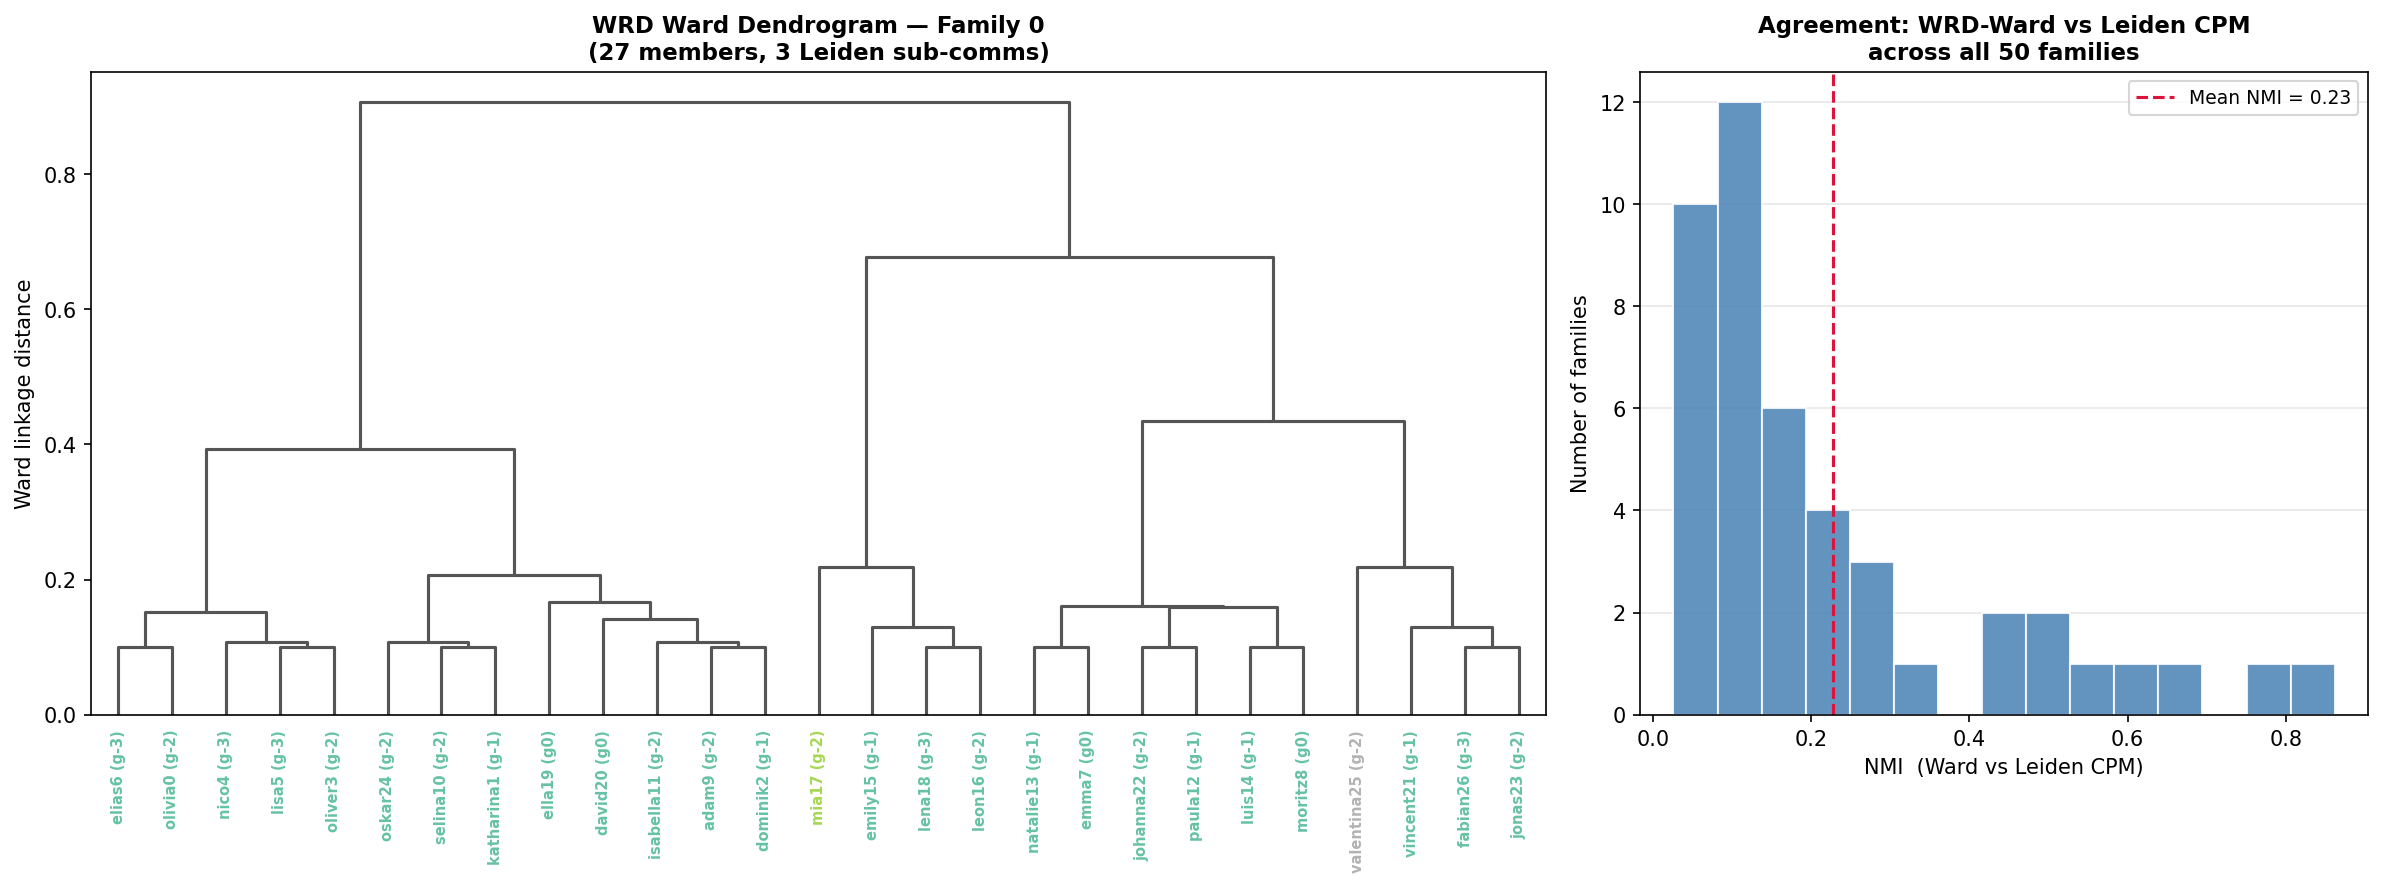
\includegraphics[width=0.95\textwidth]{task2/wrd_ward_vs_leiden.png}
\caption{Left: WRD average-linkage dendrogram for one family, leaf labels
coloured by Leiden CPM sub-community. Right: distribution of NMI between
the two methods across all 50 families --- centred well below 1.0.}
\end{figure}

\section{Cross-Family Structural Profiles}

Ranking all 50 families by ``tightness'' (mean pairwise WRD): mean WRD
ranges from 0.224 (tightest, Family 48) to 0.330 (loosest, Family 43).
Correlation between generational span and tightness is weak
($r = 0.21$, $p = 0.138$, not statistically significant) --- tightness
depends more on the density and closeness of internal relationships than
on how many generations a family spans.

\begin{figure}[h]
\centering
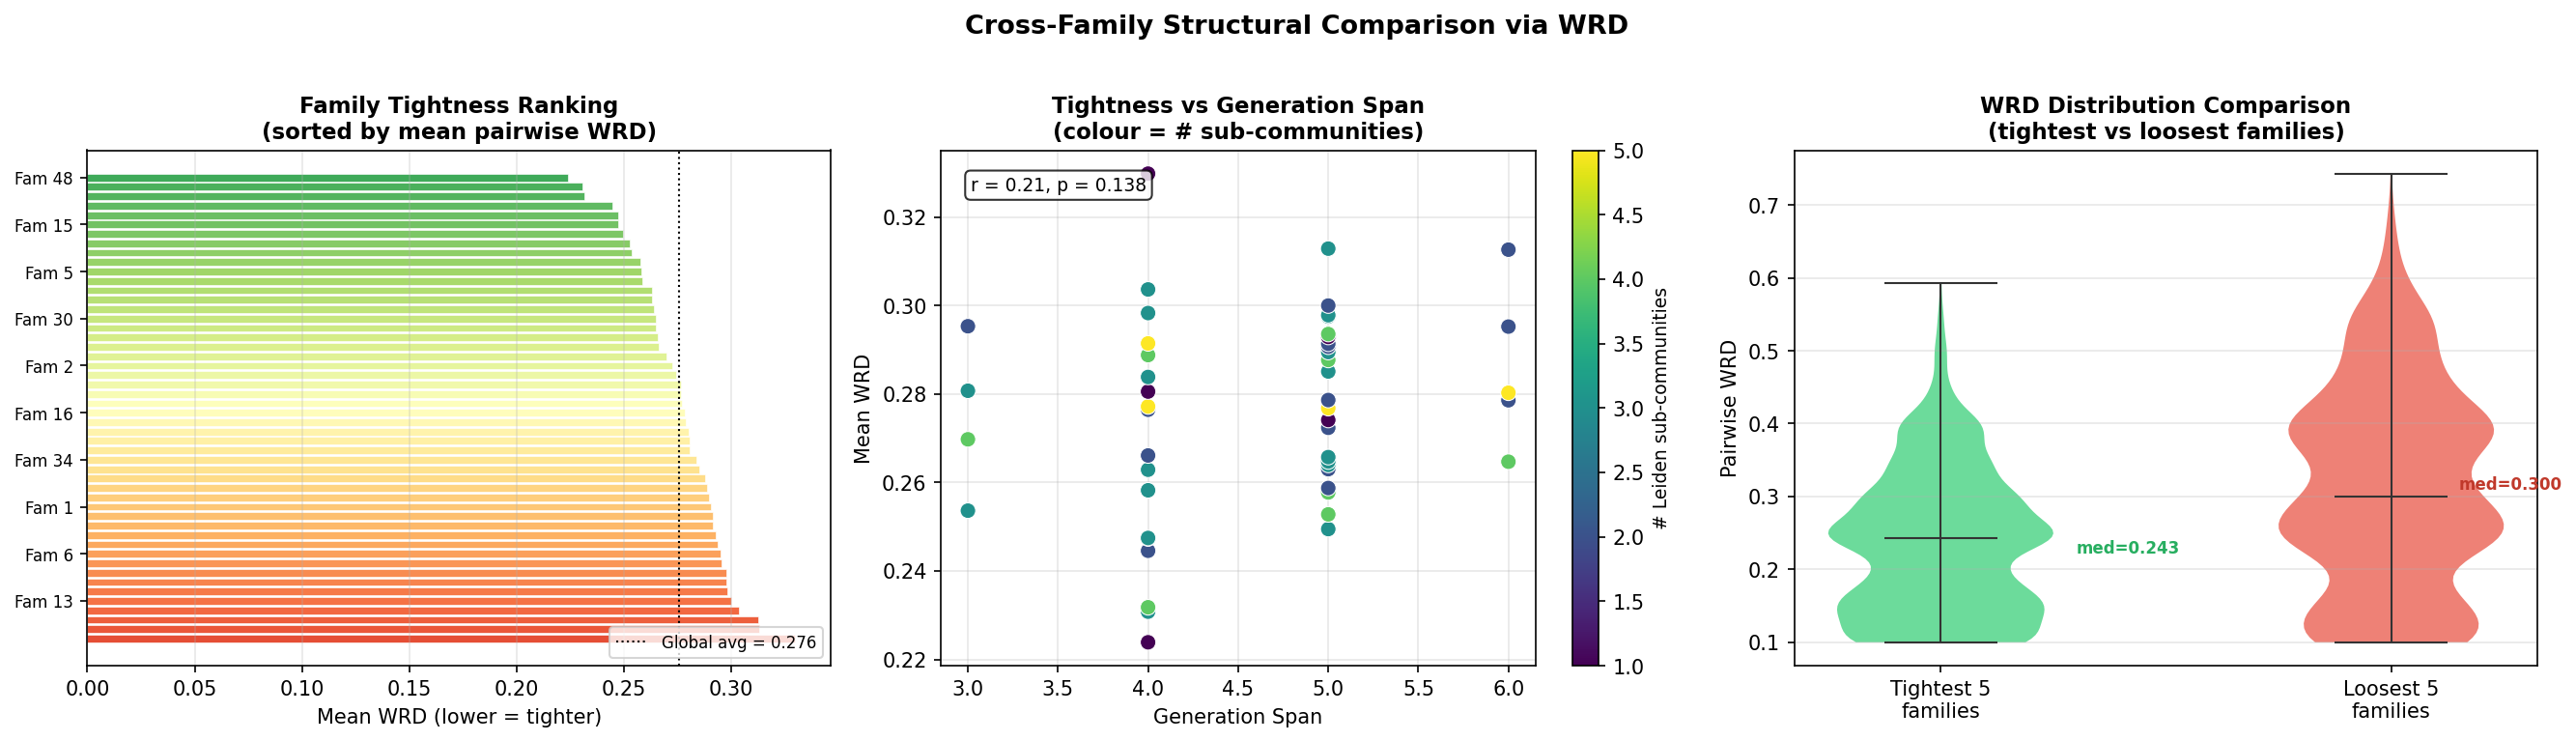
\includegraphics[width=0.95\textwidth]{task2/cross_family_wrd_profiles.png}
\caption{Family tightness ranking, tightness vs.\ generation span
(coloured by sub-community count), and a violin comparison of the
tightest vs.\ loosest 5 families.}
\end{figure}

\section{Conclusion}

Standard algorithms work: Louvain, Leiden, and Node2Vec all perfectly
separate the 50 disconnected families, and Girvan--Newman would too,
trivially, without needing to be run (\S4.2). Leiden is the best choice
for sub-groups: it reliably distinguishes a family's ``core'' from its
peripheral, low-degree members, and guarantees every community it returns
is internally connected.

WRD is not ``the true metric'' of familial relatedness --- there is no
ground-truth relatedness score to be true \emph{against} here, and the
only validation performed (agreement with Leiden's sub-communities) gave
a NMI around 0.31, i.e.\ real but partial agreement, not confirmation.
What can honestly be claimed is narrower and, I think, still
interesting: WRD \textbf{separates relationship types that hop count
collapses} (siblings vs.\ second cousins, both ``1 hop''), and it
surfaces a \textbf{hierarchical} structure (via the dendrogram) that a
flat partitioning method structurally cannot express. Whether that
hierarchy corresponds to anything a family would recognise as ``true''
would need external validation this project does not have.

% ================================================================== TASK 3
\starttask{Task 3 --- Rule Mining}

\section{Introduction \& Objective}

This task has two sub-goals:

\begin{itemize}[leftmargin=1.4em,itemsep=2pt]
\item \textbf{Rule discovery:} find patterns such as ``son of my mother's
      sister $\Rightarrow$ nephew of that aunt.''
\item \textbf{Relationship inference:} I was genuinely unclear on what
      relation labels like \rel{firstCousinOnceRemoved} and
      \rel{secondAunt/Uncle} mean, so I resolved them by testing
      competing hypotheses against the data. Google gives two different
      definitions for \rel{firstCousinOnceRemoved}, and I had never heard
      the term \rel{secondAunt/Uncle} before this dataset.
\end{itemize}

\section{Method Followed}

\subsection{Rule evaluation metrics}

\textbf{Support:} number of $(X,Z)$ pairs where the rule body holds and
the head relation also holds. \textbf{Body count:} total $(X,Z)$ pairs
satisfying the rule body, regardless of the head. \textbf{Confidence:}
support divided by body count.

\subsection{Rule mining engine}

For 2-hop rules $(X, r_1, Y) \wedge (Y, r_2, Z) \Rightarrow (H, r_{\text{head}}, T)$:
collect all $(X,Y)$ pairs satisfying $r_1$; for each, find all $Z$ with
$(Y, r_2, Z)$; check whether $(X, r_{\text{head}}, Z)$ or
$(Z, r_{\text{head}}, X)$ exists; compute support and confidence for
whichever direction is being tested. Some rules predict the $XZ$
direction, others $ZX$ --- the engine explicitly tests both rather than
assuming one.

\section{MY Rules! (hand-crafted rules)}

I designed the following rules to exercise the mining engine and check my
own understanding of the schema:

\begin{center}
\begin{tabular}{clrr}
\toprule
\textbf{\#} & \textbf{Rule} & \textbf{Confidence} & \textbf{Support} \\
\midrule
R1 & \rel{sonOf} $\wedge$ \rel{motherOf} $\Rightarrow$ \rel{brotherOf} & 100\% & 307 \\
R2 & \rel{brotherOf} $\wedge$ \rel{sisterOf} $\Rightarrow$ \rel{brotherOf} & 100\% & 324 \\
R3 & \rel{nephewOf} $\wedge$ \rel{fatherOf} $\Rightarrow$ \rel{girlCousinOf} & 47.8\% & 65 \\
R4 & \rel{nieceOf} $\wedge$ \rel{motherOf} $\Rightarrow$ \rel{boyCousinOf} & 46.5\% & 100 \\
R5 & \rel{sonOf} $\wedge$ \rel{daughterOf} $\Rightarrow$ \rel{grand*Of} & 100\% & 194 \\
R6 & \rel{sonOf} $\wedge$ \rel{girlCousinOf} $\Rightarrow$ \rel{secondAuntOf} & 51.4\% & 18 \\
R7 & \rel{grandsonOf} $\wedge$ \rel{brotherOf} $\Rightarrow$ \rel{greatUncleOf} & 34.6\% & 54 \\
R8 & \rel{granddaughterOf} $\wedge$ \rel{sisterOf} $\Rightarrow$ \rel{greatAuntOf} & 60.2\% & 50 \\
\bottomrule
\end{tabular}
\end{center}

\textbf{Why some rules hit 100\% and others hover near 50\%: gender
leakage, not noise.} R1's body starts with \rel{sonOf}, which guarantees
$X$ is male; the conclusion \rel{brotherOf} also requires $X$ male. The
constraint is already satisfied by the body, so the rule is airtight.
R3's body ends in \rel{fatherOf}, which says nothing about the child's
gender --- fathers have sons and daughters roughly equally --- but the
conclusion \rel{girlCousinOf} needs $Z$ female. The rule is right about
half the time: 47.8\%, a coin flip, exactly as the gender-leakage
explanation predicts. R8 (60.2\%) beats R7 (34.6\%) because
\rel{granddaughterOf} $\wedge$ \rel{sisterOf} happens to carry more
gender information than \rel{grandsonOf} $\wedge$ \rel{brotherOf}. Low
confidence here does not mean a bad rule --- it means a rule that is
\emph{logically correct but under-specified}: the schema has no way to
state the needed gender constraint.

\section{Relationship Semantics Inference}

\subsection{What does \texttt{firstCousinOnceRemoved} mean?}

Two hypotheses: (A) your parent's first cousin (one generation above
you), or (B) your cousin's child (one generation below you). Testing both
by mining rules in both $XZ$ and $ZX$ directions:

\begin{center}
\begin{tabular}{lccc}
\toprule
\textbf{Hypothesis} & \textbf{Direction} & \textbf{Confidence} & \textbf{Support} \\
\midrule
A: parent's cousin (\rel{sonOf} $\wedge$ \rel{boyCousinOf}) & XZ & 100\% & 64/64 \\
B: cousin's child (\rel{boyCousinOf} $\wedge$ \rel{fatherOf}) & XZ/ZX & 0\% & 0/69 \\
\bottomrule
\end{tabular}
\end{center}

\textbf{Conclusion:} \rel{firstCousinOnceRemoved} means ``my parent's
first cousin,'' stored as (younger person, \rel{firstCousinOnceRemovedOf},
older person). This is the empirical result Task 1 relies on to set the
generation weight for this relation to $-1$, not $0$ (\S2.2 in Task 1).

\subsection{What does \texttt{secondAunt/Uncle} mean?}

Rule \rel{sonOf} $\wedge$ \rel{boyCousinOf} $\Rightarrow$
\rel{secondUncleOf} (direction $ZX$): confidence 54.7\%, and similarly
for \rel{secondAuntOf}. \textbf{Conclusion:} \rel{secondAunt/Uncle}
refers to a parent's cousin; confidence sits near 50\% for the same
gender-ambiguity reason as R3/R4 above, not because the semantic
conclusion is shaky.

\section{Automated Rule Discovery}

Systematically scanning all $(r_1, r_2, r_{\text{head}})$ combinations
with minimum support 10 and minimum confidence 80\%: 264 rules
discovered, 213 (80.7\%) at 100\% confidence, 252 non-trivial (i.e.\ not
$r_1 = r_2 = r_{\text{head}}$).

\textbf{Key insight:} the extremely high proportion of 100\%-confidence
rules confirms the MetaFam knowledge graph is highly compositional and
logically consistent --- most 2-hop compositions that look like they
should determine a relation, do.

\section{Visualizations}

\begin{figure}[h]
\centering
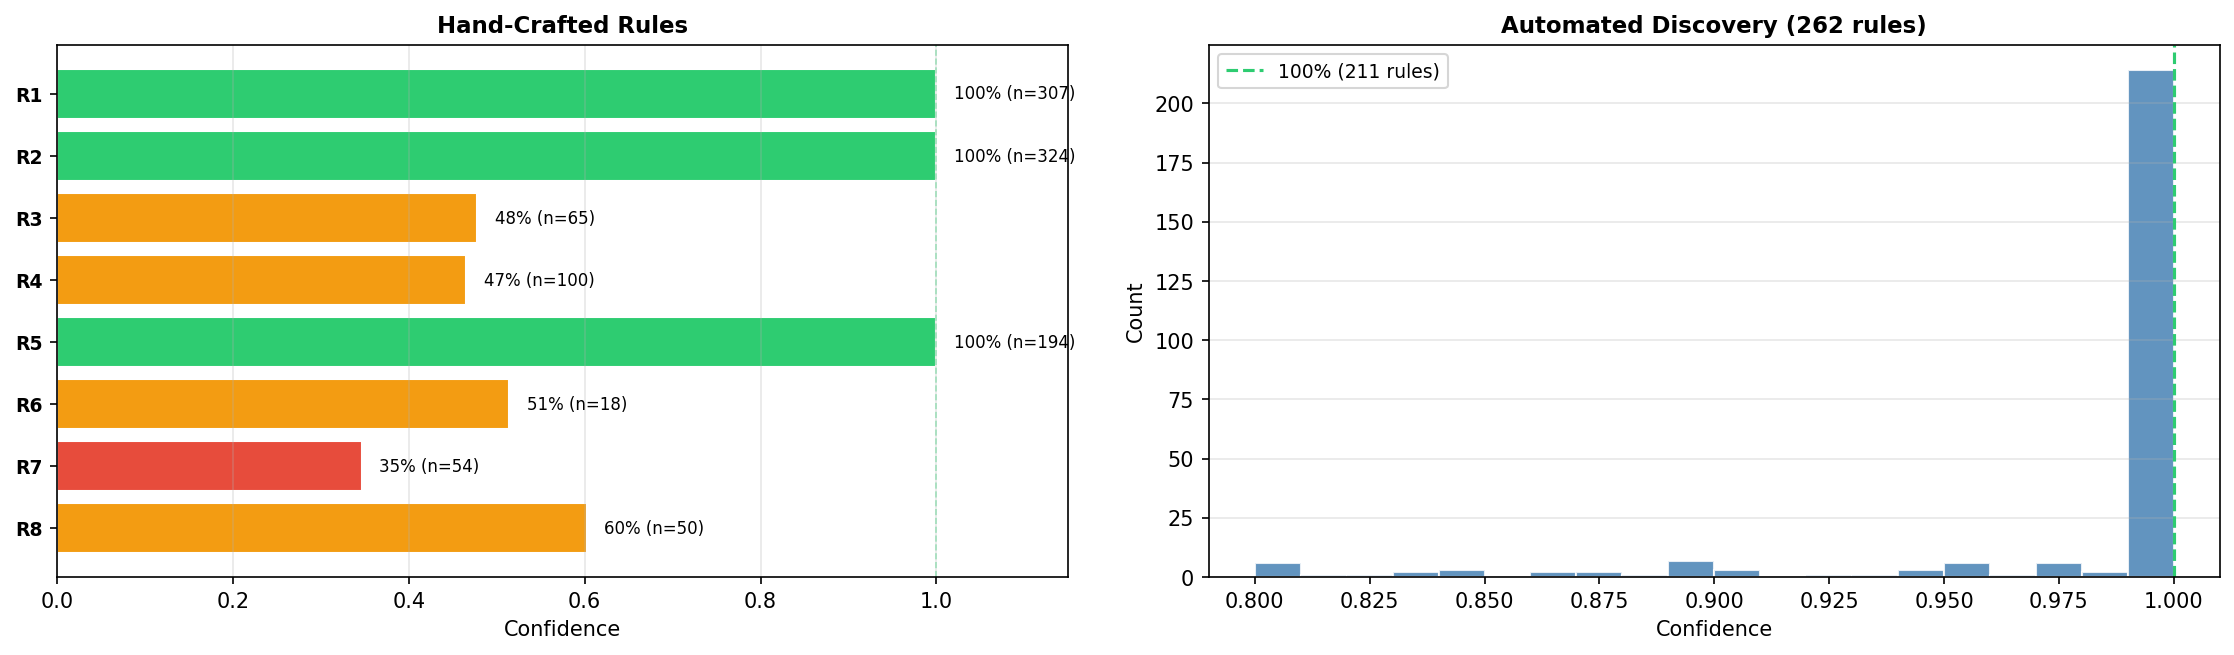
\includegraphics[width=0.95\textwidth]{task3/rule_mining_overview.png}
\caption{Confidence of the hand-crafted rules R1--R8 (left) and the full
distribution of confidences across all automatically discovered rules
(right).}
\end{figure}

\begin{figure}[h]
\centering
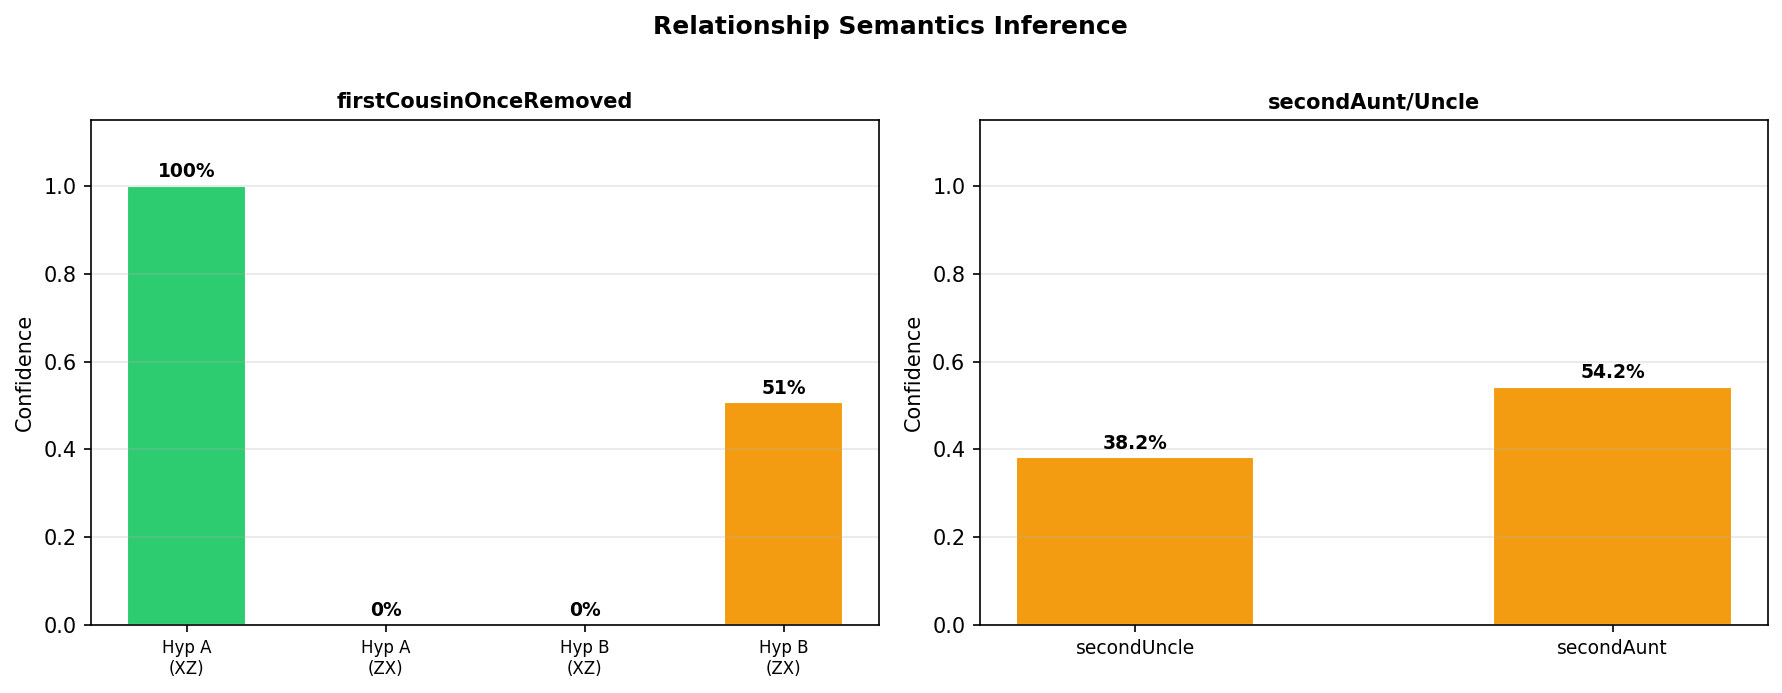
\includegraphics[width=0.85\textwidth]{task3/relationship_inference.png}
\caption{Confidence comparison for the two relationship-semantics
hypotheses (\rel{firstCousinOnceRemoved}, \rel{secondAunt/Uncle}) across
both tested directions.}
\end{figure}

\section{Key Takeaways}

\begin{itemize}[leftmargin=1.4em,itemsep=3pt]
\item \textbf{Logical consistency:} 213 of 264 automatically discovered
      rules achieve 100\% confidence.
\item \textbf{Gender filtering is the deciding factor} for whether a rule
      hits 100\% or plateaus near 50\% --- not noise in the data.
\item \textbf{Relationship semantics resolved unambiguously,} by testing
      hypotheses against data rather than guessing from the name.
\item \textbf{Rule mining enables high-confidence link inference} in this
      knowledge graph, and directly informed a data fix used in Task 1
      (\S2.2's generation-weight correction).
\end{itemize}

% ================================================================== TASK 4
\starttask{Task 4 --- Link Prediction}

\section{Objective}

Predict missing edges in the graph. The notebook implements and compares
three approaches:

\begin{itemize}[leftmargin=1.4em,itemsep=2pt]
\item \textbf{Method A --- R-GCN + DistMult} (GNN-based): learns entity
      embeddings via relation-specific message passing, scores triples
      with a bilinear function.
\item \textbf{Method B --- TransE} (KG embedding): models relations as
      translations, $\mathbf{h}+\mathbf{r}\approx\mathbf{t}$.
\item \textbf{Method C --- TransE + family-aware negative sampling} (KG
      embedding + domain knowledge): same TransE model, but with hard
      negatives sampled from within the same family, using the family
      structure discovered in Tasks 1--2.
\end{itemize}

\begin{why}
\textbf{An important limitation, stated up front rather than left for a
reader to notice.} Although every model \emph{trains} on all 28 relation
types, \texttt{test.txt} contains only \textbf{four}: \rel{sonOf} (214),
\rel{daughterOf} (200), \rel{motherOf} (88), \rel{fatherOf} (88) --- all
immediate parent/child links. Every metric in this section is therefore
measured on those four relations only. That is why the per-relation chart
(\S6) has exactly four bars, and it means a claim like ``R-GCN captures
complex multi-relational patterns'' is not directly evidenced by this
benchmark --- the harder lateral/multi-hop relations (siblings, cousins,
aunts/uncles, \ldots) that make up most of the graph are never scored
here.
\end{why}

\section{Data Setup}

\begin{center}
\begin{tabular}{lr}
\toprule
\textbf{Split} & \textbf{Triples} \\
\midrule
Train (90\% of train.txt) & 12{,}439 \\
Validation (10\% of train.txt) & 1{,}382 \\
Test (test.txt) & 590 \\
\bottomrule
\end{tabular}
\end{center}

Graph construction adds an inverse edge for every relation (e.g.\
\rel{fatherOf} $\to$ \rel{inv\_fatherOf}), giving 56 edge types and
24{,}878 directed edges in the R-GCN message-passing graph.

\begin{why}
\textbf{The train/val split is now idempotent.} The split used to shuffle
the training list \emph{in place} and reslice it, so re-running that cell
shrank the training set by another 10\% every time it was executed ---
harmless if you only run top-to-bottom once, but a silent trap otherwise.
Both splits are now derived fresh from an immutable source list every
time the cell runs.
\end{why}

\section{Evaluation Protocol}

Every model is evaluated with the standard \emph{filtered} ranking
protocol: for each test triple, rank all 1{,}316 people as candidate
heads and as candidate tails, remove other \emph{known-true} completions
from the candidate list before ranking (so a model isn't penalised for
correctly recalling a different true fact), and average the result over
head- and tail-prediction. Ties are broken \emph{pessimistically} ---
$(\text{scores} \geq \text{true score}).\text{sum()}$ counts a tied score
against the model, giving the worst-case rank rather than the best-case
one. This is a standard, defensible convention, but it is not universal,
so it is stated here explicitly rather than left implicit: results from
this notebook are not directly comparable to a paper using a different
tie-break without checking which one it reports.

\section{Method A: R-GCN + DistMult}

\subsection{Architecture}

2-layer R-GCN encoder with basis decomposition (10 bases, so the 56
relation-specific weight matrices share statistical strength instead of
each being fit independently), hidden dimension 200, dropout 0.2 ---
applied only after the non-final layers, so the embeddings actually fed
to the decoder are not additionally noised by dropout on the way out.
DistMult bilinear decoder. 1{,}150{,}320 trainable parameters.

Training: Adam (lr 0.01), \textbf{weight\_decay $=10^{-5}$ is the only L2
term} --- an earlier version of this code added a second, separate
manual L2 penalty on top of Adam's weight decay; at the scale it was set
($\approx 7.6\times 10^{-6}$ effective contribution), it was doing almost
nothing except duplicating the optimizer's own regularisation, so it has
been removed rather than kept as redundant complexity. 10 negatives per
positive, margin ranking loss (margin 1.0), batch size 1{,}024, 150
epochs, gradient clipping at norm 1.0.

\begin{why}
\textbf{The negative-sampling fix that changes every number in this
section.} Negatives were generated by \emph{tiling} the positive batch
(\rel{[a,b,c] $\to$ [a,b,c,a,b,c]}) but paired against the loss by
\emph{blocking} it (\rel{[a,b,c] $\to$ [a,a,b,b,c,c]}). The result: each
positive triple was contrasted against corruptions of \emph{other}
positives in the batch, often carrying a different relation entirely.
Margin loss still trained something under this scheme --- a coarse,
global ``all positives above all negatives'' objective --- which is why
the original models learned at all, but it is not the per-triple
contrastive objective the code intended, and it specifically degrades the
fine-grained discrimination that Hits@1 measures. Fixing the pairing
(negatives now built with \texttt{repeat\_interleave}, matching how
positives are expanded for the loss) and retraining moved every number in
this section, Hits@1 most of all.
\end{why}

\subsection{Training Dynamics}

The model converges within the first 10--20 epochs and then oscillates
around a plateau (validation MRR moving between roughly 0.55 and 0.71
across the remaining epochs) rather than smoothly improving or smoothly
overfitting --- consistent with a fairly high learning rate (0.01, held
constant by the plateau scheduler for the whole run) on a small dataset.
The best checkpoint (by validation MRR, 0.7127) is kept rather than the
final one.

\begin{figure}[h]
\centering
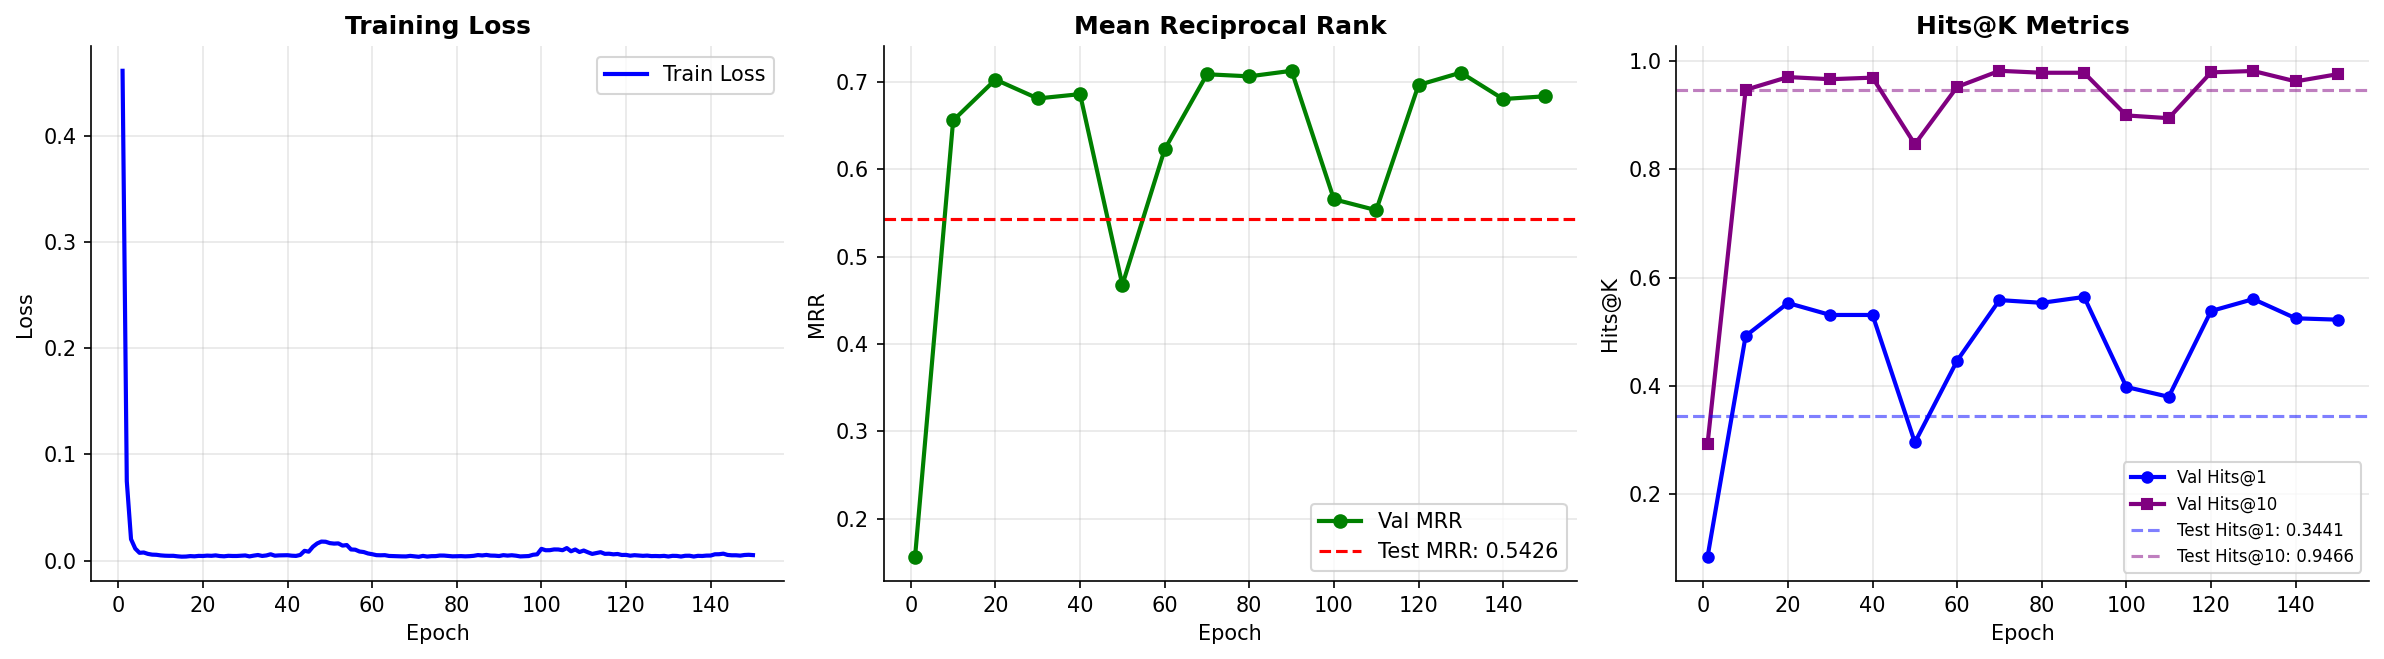
\includegraphics[width=\textwidth]{task4/rgcn_training_curves.png}
\caption{R-GCN training loss, validation MRR, and Hits@K over 150
epochs. The best-validation checkpoint (dashed line) is what gets
evaluated on the test set.}
\end{figure}

\subsection{Test Results}

\begin{center}
\begin{tabular}{lr}
\toprule
\textbf{Metric} & \textbf{Value} \\
\midrule
MRR & 0.5426 \\
Hits@1 & 34.41\% \\
Hits@3 & 67.80\% \\
Hits@10 & 94.66\% \\
Mean Rank & 4.6 \\
\bottomrule
\end{tabular}
\end{center}

The correct entity appears in the top 10 candidates 94.7\% of the time,
and in the top 3 candidates more than two-thirds of the time. A mean rank
of 4.6 (out of 1{,}316 candidates) means the correct answer is typically
among the first five.

\subsection{Per-Relation Breakdown}

\begin{center}
\begin{tabular}{lrrrr}
\toprule
\textbf{Relation} & \textbf{Count} & \textbf{MRR} & \textbf{Hits@1} & \textbf{Hits@10} \\
\midrule
fatherOf & 88 & 0.643 & 47.73\% & 98.30\% \\
motherOf & 88 & 0.553 & 34.09\% & 98.30\% \\
sonOf & 214 & 0.527 & 32.01\% & 95.33\% \\
daughterOf & 200 & 0.511 & 31.25\% & 90.75\% \\
\bottomrule
\end{tabular}
\end{center}

\begin{figure}[h]
\centering
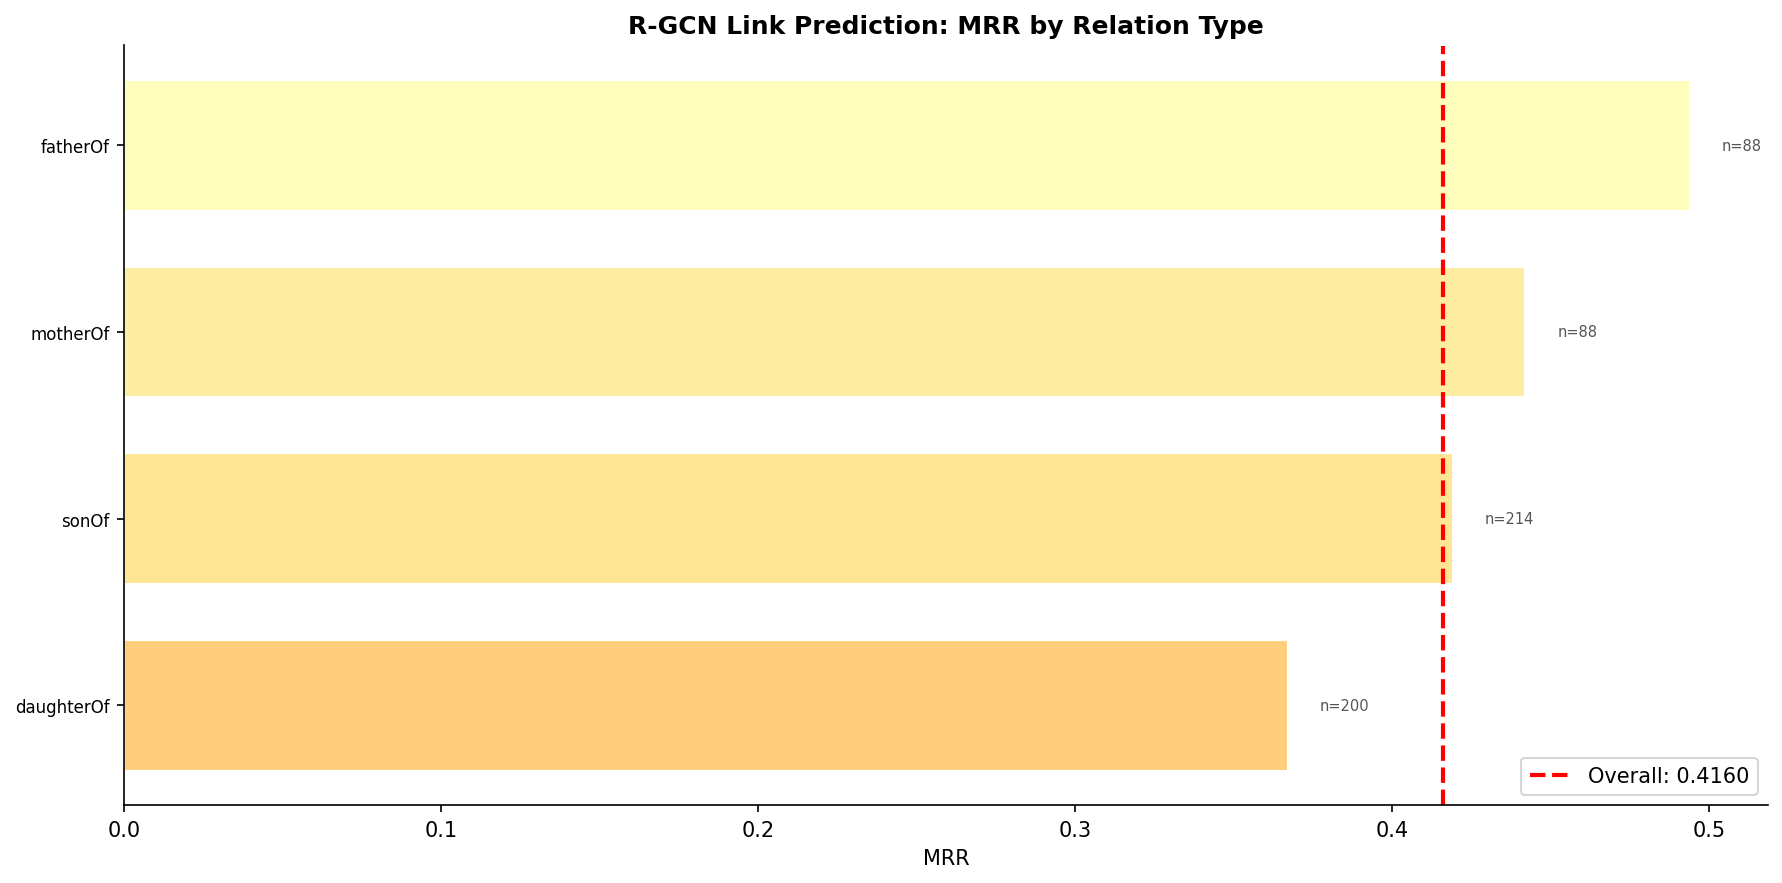
\includegraphics[width=0.85\textwidth]{task4/rgcn_per_relation_mrr.png}
\caption{R-GCN MRR by relation type. All four bars are parent/child
relations (\S1) --- there is no sibling, cousin, or multi-hop relation in
the test set to compare against.}
\end{figure}

\textbf{Insight:} parent-to-child relations are easier to predict than
child-to-parent relations. Each person has exactly 2 parents but
potentially many children, so predicting a parent is a lower-entropy
guess than predicting a child.

\section{Method B: TransE (Baseline)}

\subsection{Architecture}

Separate learned embeddings for entities and relations, embedding
dimension 200, L1 (Manhattan) distance norm, 268{,}800 trainable
parameters --- about $4.3\times$ fewer than R-GCN. Adam (lr 0.01), 10
negatives per positive (random corruption), margin ranking loss (margin
1.0), 200 epochs, entity embeddings re-normalised to unit L2 norm after
every batch.

\subsection{Test Results}

\begin{center}
\begin{tabular}{lr}
\toprule
\textbf{Metric} & \textbf{Value} \\
\midrule
MRR & 0.2854 \\
Hits@1 & 2.37\% \\
Hits@3 & 43.14\% \\
Hits@10 & 83.56\% \\
Mean Rank & 9.2 \\
\bottomrule
\end{tabular}
\end{center}

TransE reaches a respectable Hits@10 but a very low Hits@1. This is the
known structural limitation of a translational model on one-to-many
relations: a single relation vector $\mathbf{r}$ has to satisfy
$\mathbf{h}+\mathbf{r}\approx\mathbf{t}$ for \emph{every} valid tail $t$
simultaneously, so if a person has several children, TransE compromises
by placing all of them near each other rather than distinguishing them.
It lands in the right neighbourhood almost always (Hits@10) but rarely
resolves the exact individual (Hits@1).

\section{Method C: TransE + Family-Aware Negative Sampling}

\subsection{Motivation}

From Tasks 1--2: the graph is 50 disjoint family components. Standard
random negative sampling often produces trivially-wrong negatives from a
completely different family --- an ``easy'' negative that teaches the
model to distinguish families rather than to predict correctly
\emph{within} one. Family-aware sampling generates harder negatives by
drawing 70\% of them from within the same family as the positive triple
(30\% remain uniformly random).

\subsection{Family Structure}

50 family components identified from the training graph, sizes ranging
25--27. One entity out of 1{,}316 is not covered by this family mapping
--- it loses every edge once the validation split is removed from the
training graph used to build these components --- and is handled
explicitly by falling back to a uniform-random negative for it, rather
than relying on a silent dictionary-default.

\subsection{Test Results}

\begin{center}
\begin{tabular}{lr}
\toprule
\textbf{Metric} & \textbf{Value} \\
\midrule
MRR & 0.1860 \\
Hits@1 & 8.05\% \\
Hits@3 & 21.27\% \\
Hits@10 & 38.64\% \\
Mean Rank & 68.7 \\
\bottomrule
\end{tabular}
\end{center}

\subsection{Comparison with Standard TransE, and an honest reversal}

\begin{center}
\begin{tabular}{lcc}
\toprule
& \textbf{Random negatives} & \textbf{Family-aware negatives} \\
\midrule
MRR & \textbf{0.285} & 0.186 \\
Hits@1 & 2.37\% & \textbf{8.05\%} \\
Hits@3 & \textbf{43.14\%} & 21.27\% \\
Hits@10 & \textbf{83.56\%} & 38.64\% \\
Mean Rank & \textbf{9.2} & 68.7 \\
\bottomrule
\end{tabular}
\end{center}

\begin{why}
\textbf{This result changed, and not in the flattering direction, once
the negative-sampling pairing bug (\S3) was fixed --- and the honest
thing to do is report that plainly rather than keep the old framing.} An
earlier (buggy) run of this exact experiment showed a trade-off story:
Hits@1 up by roughly $32\times$, everything else down. With negatives
correctly paired to their positives, family-aware sampling instead comes
out \textbf{worse on every metric except Hits@1}, and even the Hits@1
gain is far more modest (2.37\% $\to$ 8.05\%, roughly $3.4\times$, not
$32\times$).

The likely reason the story changed: under the pairing bug, each ``hard''
negative was actually being contrasted against the wrong positive most of
the time, which diluted the family-aware signal into something closer to
the same coarse global objective TransE and R-GCN were both training
under in \S3--\S4. With correct pairing, the model is genuinely trained
almost exclusively on hard, same-family negatives from epoch 1, and 200
epochs at this capacity is not enough to solve that harder objective well
--- it learns to discriminate somewhat better within a family (the
Hits@1 gain) at a large cost to everything else, including badly
miscalling entities from \emph{other} families it was rarely shown as
negatives during training. The lesson is not ``hard negatives don't
work''; it is that hard-negative-only training needs either a mix of easy
and hard negatives, more capacity, or a curriculum (start easy, get
harder) --- and that a negative result with a clear diagnosis is worth
keeping in the writeup, not quietly deleting.
\end{why}

\section{Final Comparison: All Methods}

\begin{center}
\begin{tabular}{lrrrrr}
\toprule
\textbf{Model} & \textbf{MRR} & \textbf{Hits@1} & \textbf{Hits@3} & \textbf{Hits@10} & \textbf{Params} \\
\midrule
R-GCN + DistMult & \textbf{0.543} & \textbf{34.41\%} & \textbf{67.80\%} & \textbf{94.66\%} & 1{,}150{,}320 \\
TransE (random negatives) & 0.285 & 2.37\% & 43.14\% & 83.56\% & 268{,}800 \\
TransE (family-aware negatives) & 0.186 & 8.05\% & 21.27\% & 38.64\% & 268{,}800 \\
\bottomrule
\end{tabular}
\end{center}

\begin{figure}[h]
\centering
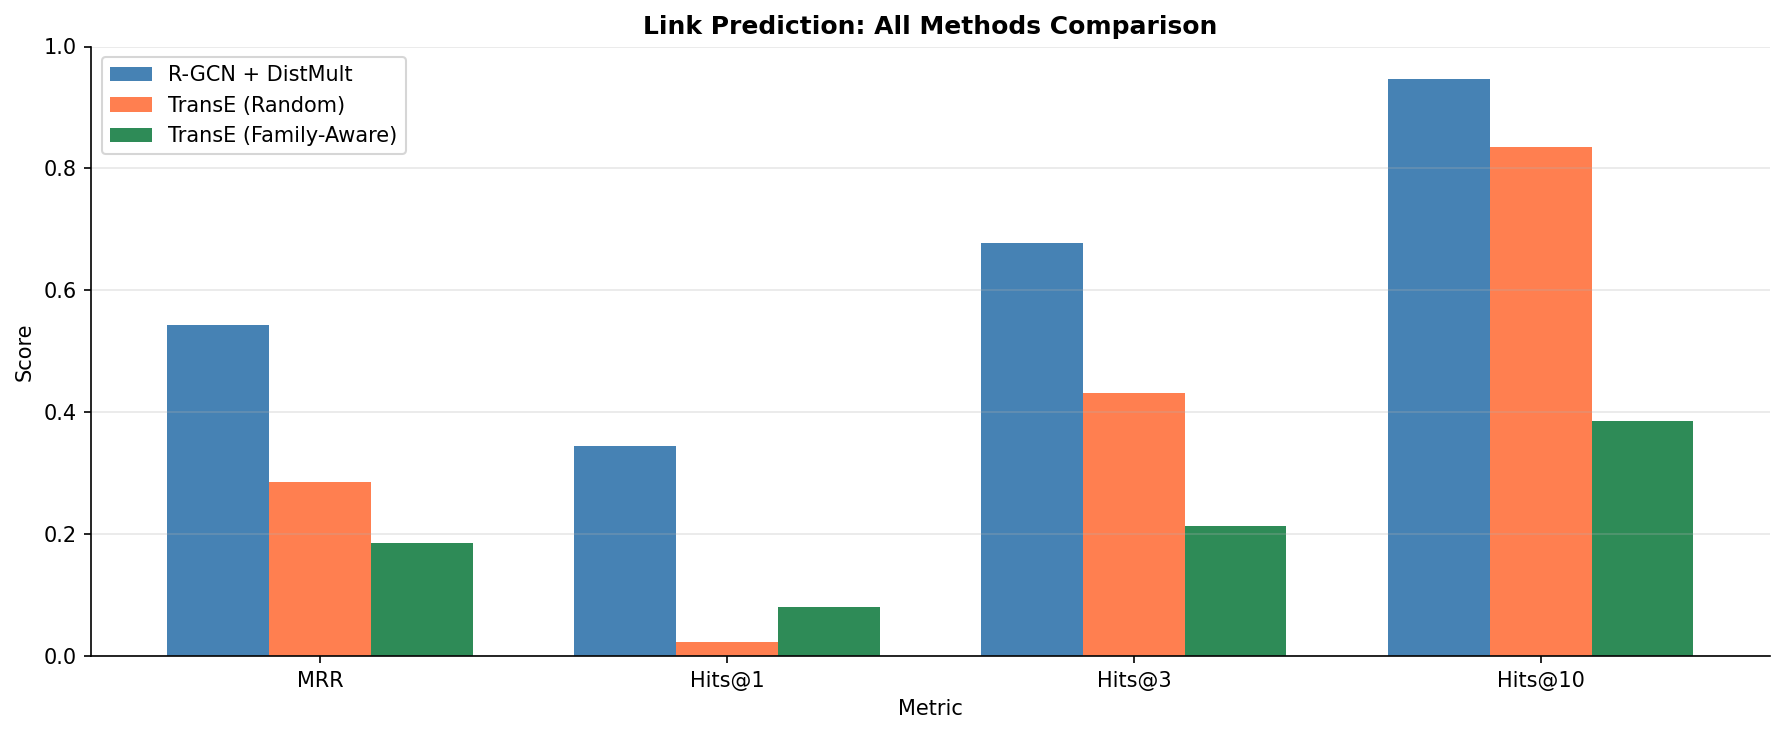
\includegraphics[width=0.92\textwidth]{task4/all_methods_comparison.png}
\caption{All three link-prediction approaches side by side, on the four
parent/child relations that \texttt{test.txt} covers (\S1).}
\end{figure}

\begin{figure}[h]
\centering
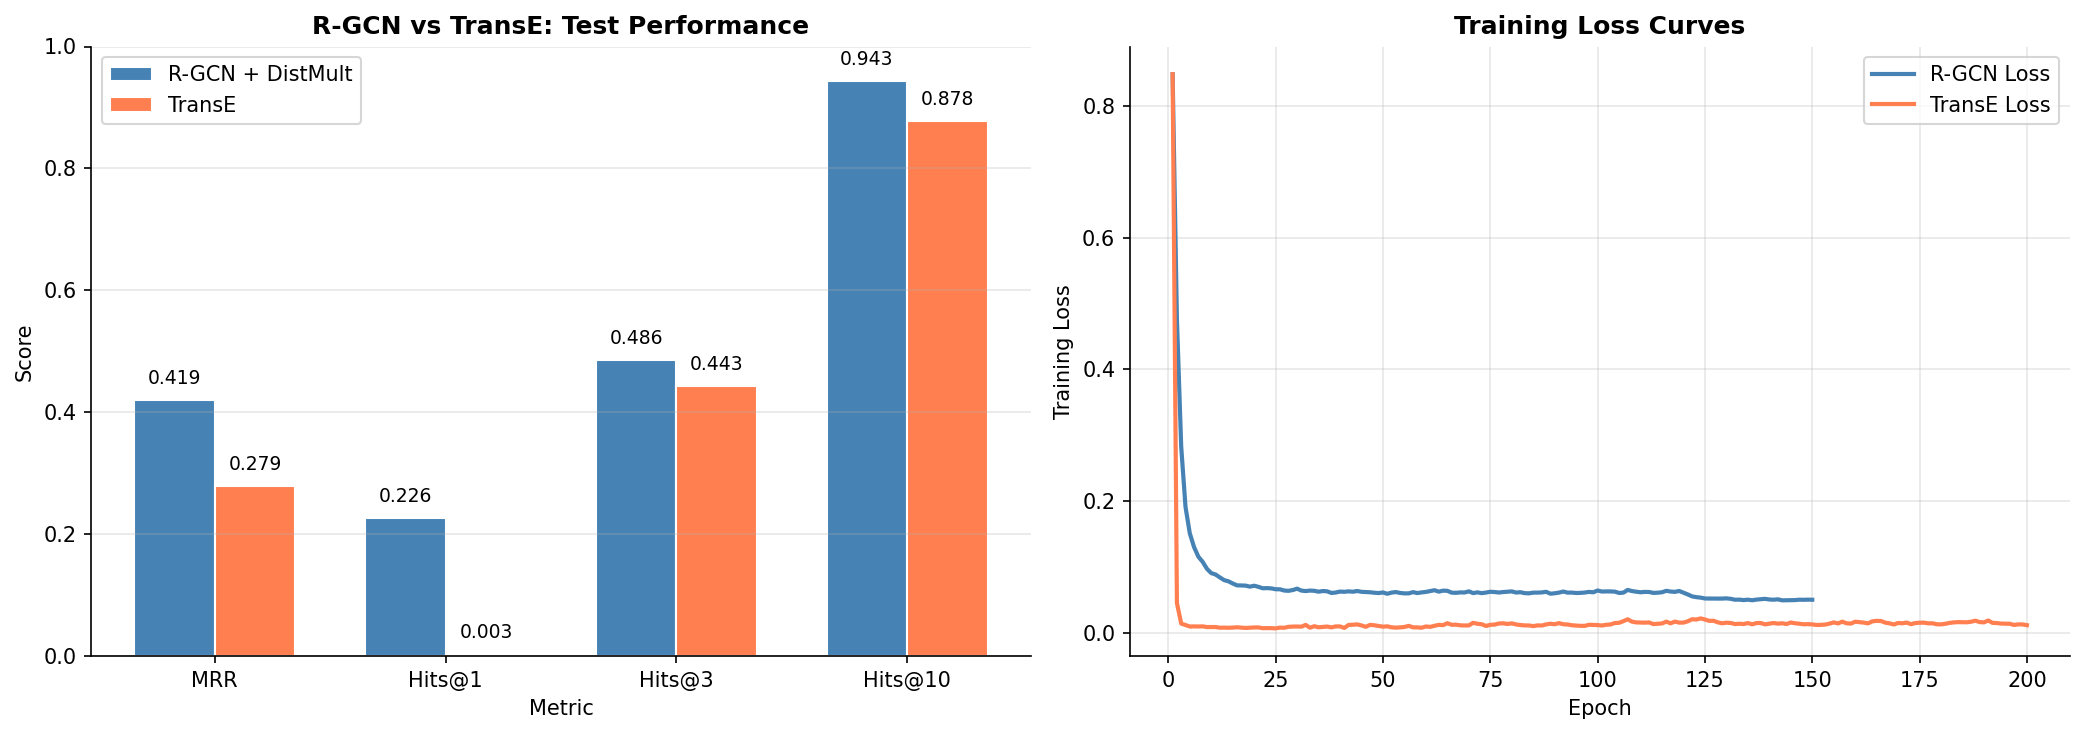
\includegraphics[width=0.92\textwidth]{task4/rgcn_vs_transe_comparison.png}
\caption{R-GCN vs.\ TransE (random negatives): metric-by-metric bars and
training-loss curves side by side.}
\end{figure}

\textbf{R-GCN wins decisively, on every metric, not just on average.} The
Hits@1 gap (34.4\% vs.\ 2.4\%) is the sharpest evidence: TransE almost
never lands the exact right answer, though it usually lands in the right
neighbourhood (Hits@10 83.6\%) --- exactly the one-to-many blurring
predicted in \S4. R-GCN, which learns a separate message-passing
transformation per relation type and aggregates neighbourhood
information rather than relying on one global translation vector per
relation, resolves the individual far more often.

\section{Key Findings \& Analysis}

\begin{itemize}[leftmargin=1.4em,itemsep=3pt]
\item \textbf{R-GCN dominates} on every reported metric. It captures the
      compositional structure that Task 3's rule mining independently
      showed the graph has (\S5 of Task 3: 213 of 264 discovered rules at
      100\% confidence) --- a graph this logically compositional is
      exactly where relation-aware message passing should have an edge
      over a single global translation vector per relation.
\item \textbf{TransE's structural limitation is real, not a tuning gap.}
      One-to-many relations (a parent with several children) cannot be
      represented by a single translation vector without blurring the
      targets together, and MetaFam is full of one-to-many relations.
\item \textbf{Domain-knowledge injection needs care, and the honest
      result here is a partial failure, not a partial success.} Sampling
      harder negatives from Task 1/2's family structure improved only
      Hits@1, and by less than initially observed once the pairing bug
      was fixed; every other metric got substantially worse. Hard
      negatives are not automatically better negatives without a mix or
      a curriculum.
\item \textbf{Connections to other tasks:} Task 1's family structure
      enabled family-aware sampling (\S7); Task 2's community detection
      validated that the family components are exactly what Task 1 found
      structurally; Task 3's rule compositionality plausibly explains
      part of why R-GCN, which can chain relation-specific
      transformations across hops, generalises better than TransE here.
\end{itemize}

\section{Saved Artifacts}

\begin{center}
\begin{tabular}{ll}
\toprule
\textbf{Model} & \textbf{Path} \\
\midrule
R-GCN + DistMult & \texttt{models/rgcn\_link\_predictor.pt} \\
TransE (random negatives, best checkpoint) & \texttt{models/transe\_best.pt} \\
\bottomrule
\end{tabular}
\end{center}

The R-GCN checkpoint stores model weights, entity/relation ID mappings,
hyperparameters, and test metrics, so it can be reloaded and re-evaluated
without retraining. \texttt{transe\_best.pt} is Method B's (random
negatives) best-validation checkpoint; Method C's (family-aware) model is
not separately persisted.

\end{document}
